\documentclass[UTF8]{ctexart}
\usepackage{ctex}

\usepackage{graphicx}

% amsmath ... are included in this package of mine.
\usepackage{MyMathPackage}

\usepackage{tikz}
% calc for calculation of the tangent of a circle.
\usetikzlibrary{calc}

\usepackage{pgfplots}
\pgfplotsset{compat=1.16}

\usepackage{chemfig}

\renewcommand{\headheight}{12.7pt}

\usepackage{fancyhdr}
\fancyhead[L]{\leftmark}
\fancyhead[R]{\emph{2020 寒假笔记}}
\fancyfoot[C]{\textbf{\thepage}}
\fancyfoot[L]{\emph{\textbf{作者:贺官羽铭}}}
\fancyfoot[R]{}

% These two package are used to create enumeration in oneline,
% to change enumeration label ...
\usepackage{enumitem}
\usepackage{multicol}

\author{贺官羽铭}
\date{\today}
\title{2020 寒假笔记}

% Until subsubsection (inclusive).
\setcounter{secnumdepth}{3}

\usepackage{hyperref}
\hypersetup{
pdftitle={2020寒假笔记},
pdfauthor={贺官羽铭},
colorlinks=true,
linkcolor=blue}

\begin{document}
\pagestyle{plain}
\pagenumbering{gobble}
\begin{tikzpicture}[remember picture, overlay]
\node[anchor=north west] at (current page.north west)
{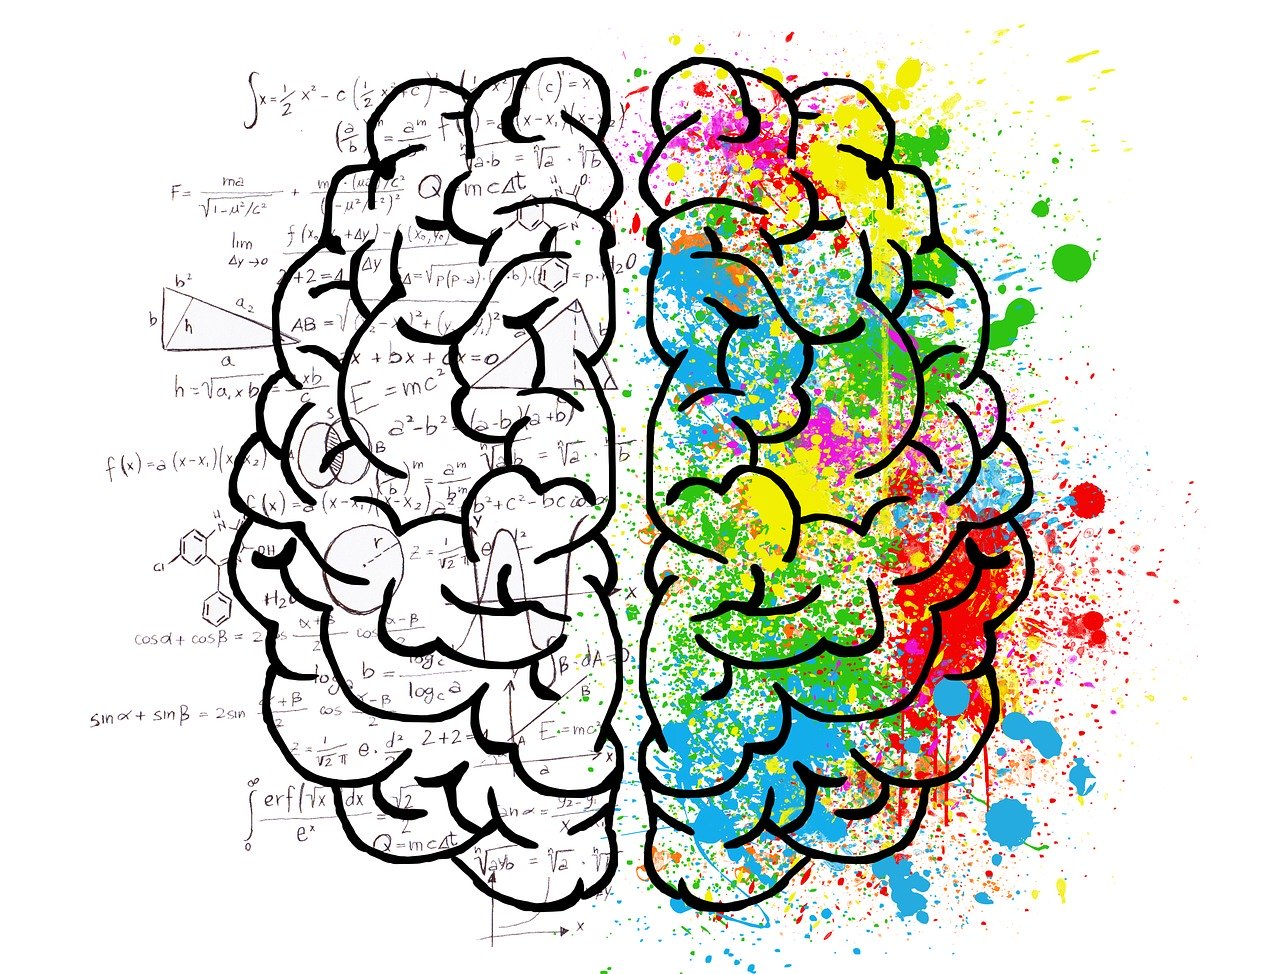
\includegraphics[height=0.35\paperheight]{Assets/brain.jpg}};
\node[anchor=south east] at (current page.south east)
{
\includegraphics[width=0.5\paperwidth]{Assets/laptop.jpg}};

\node[anchor=south east,rotate=15*rand] (B) at (current page.center) 
{\Huge \textbf{\textcolor{green}{0}}};
\node[anchor=east,rotate=15*rand] (A) at ($(B.west)+(-1.5mm,0)$)
{\Huge \textbf{\textcolor{red}{2}}};
\node[anchor=west,rotate=15*rand] (C) at ($(B.east)+(1.5mm,0)$)
{\Huge \textbf{\textcolor{yellow}{2}}};
\node[anchor=west,rotate=15*rand] (D) at ($(C.east)+(1.5mm,0)$)
{\Huge \textbf{\textcolor{blue}{0}}};

\node[anchor=north] (Title) at (current page.center) 
{\Huge \textbf{寒假笔记}};
\end{tikzpicture}

\newpage
\maketitle

\newpage
\pagenumbering{Roman}
\begin{center}
\begin{LARGE}
\textbf{献词}
\end{LARGE}

\medskip
{\large \textbf{\textcolor{green!60!black}
{谨以此笔记献给计算机科学家Donald E. Knuth。}}}
\\没有他开发的\TeX 排版软件我今天写的笔记就不会这么漂亮。
\end{center}

% Go to the bottom of the page.
\vfill
Copyright \copyright{} 2020 by 贺官羽铭.

Permission is hereby granted to copy, distribute and/or modify 
\emph{the documentation} under the terms of the \textsc{GNU} General Public License, 
Version 3.0 or any later version published by the Free Software Foundation.
A copy of the license is included in the file entitled LICENSE.

Permission is also granted to copy, distribute and/or modify 
\emph{the Corresponding Source} under the terms of the \textsc{GNU} General Public 
License, Version 3.0 or any later version published by the Free Software Foundation.
A copy of the license is included in the file entitled LICENSE.

\emph{Some images used in the documentation}, however, come from websites that 
provide free images. More information can be found in the ``COPYRIGHT'' file inside 
the ``Assets'' folder.

\newpage
\tableofcontents

\newpage
\begin{center}
\begin{LARGE}
\textbf{前言}
\end{LARGE}
\end{center}

寒假正好遇上新型冠状病毒疫情,学校提前开学的计划就被取消了。

学校搞了个网课,然而里面的内容参次不齐,以及有的确实太无聊,我想自己总结下一些知识点吧,这些知识点
基本上都是我自己从网课和各种地方筛选出来的,有的根本就不是网课的内容。所以本笔记和网课关系不是太大。
只是有的地方按照它的顺序做了下。

笔记用什么记呢?笔和纸又累又难看,OneNote...也不太好。
最终我选择了\LaTeX 帮助我记笔记,以达到最大化的视觉享受,顺便还能提高我的\LaTeX 水平。本文使用
\LaTeX 排版,用PGF/Ti\emph{k}Z生成插入的矢量图,用\\
B\textsc{ib}\TeX 生成参考文献。

笔记里包含了一些学科的一些基础知识,我对一些有趣高中问题的解法和某种类型问题的思考,网课里的
一些有趣内容,以及网课里没有的一些内容。

\medskip
\begin{center}
\begin{LARGE}
\textbf{致谢}
\end{LARGE}
\end{center}
没有人能十全十美。感谢在我成长过程中能够帮助我以及包容我的同学和朋友们,他们使我的生活更美好。尤其是
感谢那些曾经见过我的不当行为或是被我伤害过的而能够包容我并仍然愿意和我成为朋友的人,他们给了我力量。

\newpage
\pagestyle{fancy}
\pagenumbering{arabic}

\part{寒假数学:数学思想与方法}
\begin{quotation}
``\emph{学数学唯一的方式是做数学。}''

{\ttfamily ``The only way to learn mathematics is to do \\mathematics.''\\
--- Paul Halmos}

``\emph{数学就像尼罗河一样,从微不可察到浩瀚博大。}''

{\ttfamily ``The study of mathematics, like the Nile, begins \\
in minuteness but ends in magnificence.''\\
--- Charles Caleb Colton}
\end{quotation}

\section{课程:数学思想方法 -- 1 函数与方程}
\subsection{转化为方程}
网课中提到了这样一个有趣的题目:已知
\[
\frac{\sqrt{5}b - c}{5a} = 1
\],
$a,\ b,\ c \in \mathbb{R}$, 则\(b^2\)与\(4ac\)的大小关系为?

要考虑\(b^2\)与\(4ac\)的大小关系,可考察\(b^2 - 4ac\)的正负。这不是别的,正是一元二次方程的
判别式的形式。故考虑把题目中的等式转化为一元二次方程的形式。我们有:
\begin{align}
(a &\neq 0) \nonumber \\
\sqrt{5}b - c &= 5a \nonumber \\
\sqrt{5}^2a - \sqrt{5}b + c &= 0
\end{align}
即一元二次方程\(ax^2 + bx + c = 0\)在$\mathbb{R}$上至少有一个解$-\sqrt{5}$。
且由于我们的每一步转化都有必要且充分的关系,
故\(b^2 \geq 4ac\)

\subsection{更换自变量}
在一些带有参变量的一元二次不等式里,可以更换自变量,把一元二次不等式转化为线性函数来求解。
比如网课中提到的已知\(7x - 2 > (x^2 - 1)m\)对\(m \in [-2,2]\)恒成立,求实数$x$的取值范围。
把$m$作为自变量,就可以得到关于$m$的线性函数。具体做法不是我们讨论的重点,今转而证明其必要充分性。
\begin{proof}
首先题目的意思是对\(\forall m \in [-2,2]\),求$x$的集合,使其中的$x$都满足
\(7x - 2 > (x^2 - 1)m\). 我们通过更换自变量的做法得出的结果是一个$x$的集合,其中的$x$都满足
了对\(\forall m \in [-2,2]\),\(0 > (x^2 - 1)m - 7x + 2\)。由于
\(7x - 2 > (x^2 - 1)m\)与\(0 > (x^2 - 1)m - 7x + 2\)互为必要且充分的条件,故这种方法做
出来的就是解。
\end{proof}

\subsection{数列最值}
对于一个数列,考察其最值的方法也可以参照考察函数最值的方法,因为数列也可以被看成定义在整数集的某
个子集上的函数,和一般的函数来说区别只是定义域不连续。比如网课中的某道题的一部分:求
\[
\sigma_n = \sum_{i = n+1}^{2n}{\frac{1}{i}}
\]的下确界.\footnote{界的概念虽然未涉及,但比较基础,我们就直接用了。这里简单介绍下,如果某个数集
$\mathbb{S}$中的所有元素$\leq\ (\geq)$某个数$m(n)$则$m(n)$是$\mathbb{S}$的上界(下界)。
上界(下界)中如果存在最小(最大)的数$M(N)$则数$M(N)$是$\mathbb{S}$的上(下)确界。}

讨论函数最值时有时我们使用单调性判断,而单调性可通过取$x_1,x_2$做差判断,我们把这个方法运用到这
题上。令\(d = \sigma_{n+1} - \sigma_n\),考察$d$的正负。我们有
\begin{align}
d 
&= \frac{1}{2n+1} + \frac{1}{2n + 2} - \frac{1}{n + 1} \nonumber \\
&> \frac{1}{2(n + 1)} + \frac{1}{2(n + 1)} - \frac{1}{n + 1} = 0
\end{align}
就明白$\sigma_n$递增,于是其下确界是$\sigma_1 = \frac{1}{2}$.

\section{课程:数学思想方法 -- 2 函数与方程在几何中的应用}
课程中提到了这样一道题:
已知正方体的棱长为$a$,平面$\alpha$与每条棱所在直线成角都相等,$\cdots$。
课程里直接给出了一个特例平面,并说把这个平面平移,而没有讲$\alpha$是怎么被求出来的。现在我们来做一
下。

首先,让正方体一个顶点上的三条棱都放在坐标轴上,这样,显然,每条棱所在直线都和坐标轴的其中一条平行。
这样只要找到$\alpha$与三条坐标轴成的角相等就好了。这即是让它的法向量$\vec{n_{\alpha}}$与
\((0,0,1),\ (0,1,0),\ (1,0,0)\)成的角都相等。设
\[
\vec{n_{\alpha}} = (x,y,z)
\]
则$x=y=z$,便取$\vec{n_{\alpha}} = (1,1,1)$就好了。

\section{课程:数学思想方法 -- 3 构造}
\subsection{构造向量解题}
可能会遇到这种题目,给出了如下条件:
\begin{equation*}
\begin{cases}
\sin{\alpha_0} + \cdots + \sin{\alpha_n} = a \\
\cos{\alpha_0} + \cdots + \cos{\alpha_n} = b
\end{cases}
\end{equation*}
这时可构造向量\(\vec{v}_0 = (\sin{\alpha_0}, \cos{\alpha_0}), \cdots, 
\vec{v}_n = (\sin{\alpha_n}, \cos{\alpha_n})\)并做和
\(\vec{n} = \vec{v}_0 + \cdots + \vec{v}_n\)来研究。此时\(\vec{n}=(a,b)\)。

例:若
\begin{equation}
\begin{cases}
\sin{\alpha} + \sin{\beta} + \sin{\gamma} = 0 \\
\cos{\alpha} + \cos{\beta} + \cos{\gamma} = 0
\end{cases}
\label{eq:exam1}
\end{equation}
且\(0 < \alpha < \beta < \gamma < 2\pi\),求\(\beta - \alpha\)。

\textbf{解}:
令\(\vec{\varphi}_\alpha = (\sin{\alpha}, \cos{\alpha}), \cdots, 
\vec{\varphi}_\gamma = (\sin{\gamma}, \cos{\gamma})\), 
\(\vec{s} = \vec{\varphi}_\alpha + \vec{\varphi}_\beta + \vec{\varphi}_\gamma\)
则由\ref{eq:exam1}得,\(\vec{s} = \vec{0}\),或表示为
\(\vec{\varphi}_\gamma = - (\vec{\varphi}_\alpha + \vec{\varphi}_\beta)\)。
现在由这个关系推导角的关系。首先考虑一个特殊情况,当\(\gamma = \frac{3}{2}\pi\)时,如图
\ref{fig:exam1},参见各个向量的情况。

\begin{figure}[!hbtp]
\begin{center}
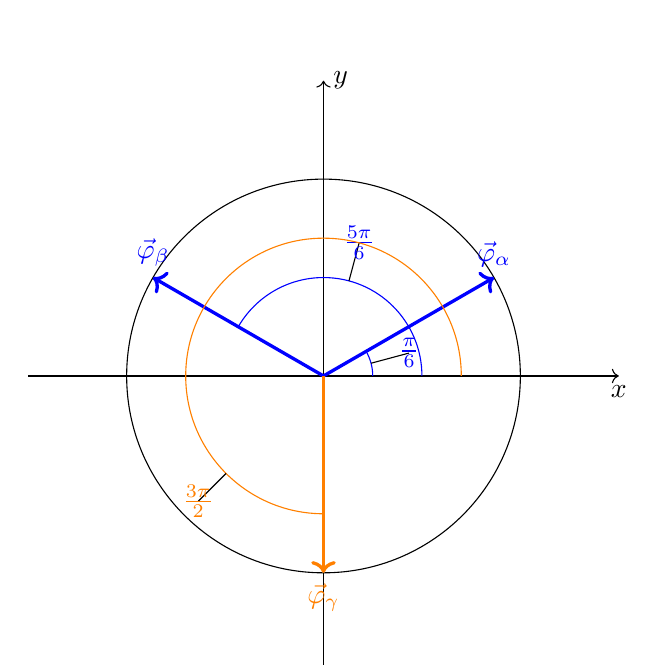
\begin{tikzpicture}[scale=2.5]
\draw[->] (-1.5,0) -- (1.5,0) node [anchor=north] {$x$};
\draw[->] (0,-1.5) -- (0,1.5) node [anchor=west] {$y$};

\draw (0,0) circle [radius=1];

\draw[color=blue, very thick, ->] (0,0) -- (30:1)
 node [anchor=south] {$\vec{\varphi}_\alpha$};
\draw[color=blue, very thick, ->] (0,0) -- (150:1)
 node [anchor=south] {$\vec{\varphi}_\beta$};
\draw[color=orange, very thick, ->] (0,0) -- (270:1) 
node [anchor=north] {$\vec{\varphi}_\gamma$};

\draw[color=blue] (2.5mm,0) arc 
[start angle=0, end angle=30, radius=2.5mm, thick];
\draw (15:2.5mm) -- +(15:2mm) node [color=blue] {$\frac{\pi}{6}$};
\draw[color=blue] (5mm,0) arc 
[start angle=0, end angle=150, radius=5mm, thick];
\draw (75:5mm) -- +(75:2mm) node [color=blue] {$\frac{5\pi}{6}$};
\draw[color=orange] (7mm,0) arc 
[start angle=0, end angle=270, radius=7mm, thick];
\draw (225:7mm) -- +(225:2mm) node [color=orange] {$\frac{3\pi}{2}$};

\end{tikzpicture}
\end{center}
\caption{
\(\vec{\varphi}_{\alpha,\beta,\gamma}\)的关系当\(\gamma = \frac{3}{2}\pi\)时}
\label{fig:exam1}
\end{figure}

这时很易看出\(\beta - \alpha = \frac{\pi}{3}\)。随后改变$\vec{\varphi}_\gamma$,
另外两向量的位置唯一确定,且相对位置不变,相当于原图旋转了一些。故无论如何
\(\beta - \alpha = \frac{\pi}{3}\)。

\subsection{构造对偶式}
我们在网课里看到了一个有趣的解法,背后的原理暂时没有弄明白,先把做法记下。

例:
试求\(\sin^2{20\mdeg} + \cos^2{50\mdeg} + 
\sin{20\mdeg}\cos{50\mdeg}\)。

\textbf{解}:

令\(\alpha = \sin^2{20\mdeg} + \cos^2{50\mdeg} + 
\sin{20\mdeg}\cos{50\mdeg}\), 把\(\alpha\)中的sin换成cos,cos换成sin,就
得到了所谓的对偶式\(\beta = \cos^2{20\mdeg} + \sin^2{50\mdeg} + 
\cos{20\mdeg}\sin{50\mdeg}\).

我们有
\begin{align}
\alpha + \beta
&= (\sin^2{20\mdeg} + \cos^2{20\mdeg}) + (\sin^2{50\mdeg} + 
\cos^2{50\mdeg}) \nonumber \\
&+ (\sin{20\mdeg}\cos{50\mdeg} + 
\cos{20\mdeg}\sin{50\mdeg}) \nonumber \\
&= 2 + \sin{70\mdeg}
\end{align}
\begin{align}
\alpha - \beta
&= (\sin^2{20\mdeg} - \cos^2{20\mdeg}) + (\sin^2{50\mdeg} - 
\cos^2{50\mdeg}) \nonumber \\
&+ (\sin{20\mdeg}\cos{50\mdeg} - 
\cos{20\mdeg}\sin{50\mdeg}) \nonumber \\
&= -\cos{40\mdeg} + \cos{100\mdeg} - 
\sin{30\mdeg}
\end{align}
注意到
\begin{align*}
\cos{40\mdeg} = \cos{(70\mdeg - 30\mdeg)}\\
\cos{100\mdeg} = \cos{(70\mdeg + 30\mdeg)}
\end{align*}
故
\begin{equation}
\alpha - \beta = -2\sin{70\mdeg}\sin{30\mdeg} - \frac{1}{2}
\end{equation}
则
\begin{align}
\alpha
&= \frac{1}{2}(\alpha + \beta + \alpha - \beta) \nonumber \\
&= \frac{3}{4}
\end{align}

我们很好奇这是不是一个特殊的例子才成立。于是我们把\(30\mdeg,\ 50\mdeg\)换成一般角\(A,\ B\),
并令
\begin{align*}
m &= \sin^2{\alpha} + \cos^2{\beta} + \sin{\alpha}\cos{\beta} \\
n &= \cos^2{\alpha} + \sin^2{\beta} + \cos{\alpha}\sin{\beta}
\end{align*}

则,很易通过之前的推导看出,
\begin{align*}
m + n &= 2 + \sin{(\alpha + \beta)} \\
m - n &= 2\sin{(\alpha - \beta)}\sin{(\alpha + \beta)} + \sin{(\alpha - \beta)}
\end{align*}

这样,只有\(2\sin{(\alpha - \beta)} = -1\)是,m才能被求出,或者当\\
\(\sin{(\alpha - \beta)},\ \sin{(\alpha + \beta)}\)都可被求出时也行。

\subsection{构造几何图形}
课程里提到了一个比较经典的题:给出一个三角形的一角和其对边,求它的面积的最大值。课程中给了构造其
外接圆的方法。首先由正弦定理,确定其一角和对边的话,其外接圆的半径便是常数了。图
\ref{fig:ConstructGeometry}展示了当定角为$\frac{\pi}{3}$,对边为2时的情况。显然,
\(S_{\triangle ABC}\)最大仅当C在最上面。

\begin{figure}[!hbtp]
\begin{center}
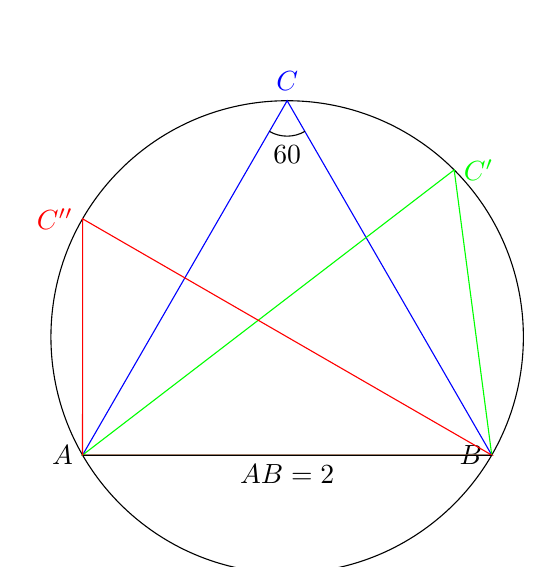
\begin{tikzpicture}[scale=1.5]
\coordinate [label=left:{$A$}] (A) at (210:2);
\coordinate [label=left:{$B$}] (B) at (-30:2);

\draw (0,0) circle [radius=2];
\draw[color=blue] (A) -- (B) -- (90:2) node[anchor=south] {$C$} -- cycle;
\draw[color=green] (A) -- (B) -- (45:2) node[anchor=west] {$C'$} -- cycle;
\draw[color=red] (A) -- (B) -- (150:2) node[anchor=east] {$C''$} -- cycle;
% make AB black.
\draw (A) -- (B);

\node[anchor=north] at (0,-1) {$AB=2$};

\draw (90:2) +(240:3mm) arc [start angle=240, end angle=300, radius=3mm];
\node[anchor=north] at (0,1.7) {$60\mdeg$};

\end{tikzpicture}
\end{center}
\caption{构造外接圆}
\label{fig:ConstructGeometry}
\end{figure}

不过构造要注意的一点,课程里没有提,就是,构造的东西是否和它唯一对应。首先,圆上这样的每一个三角形
都满足题目条件,只因弦对的圆周角相等。另一方面,任意的这样三角形都可被这样放在圆上,这比较显然。故
构造出来的东西与题目唯一对应。

这做法比较简单易懂,然而我们想转而考察纯代数求其最大值。
首先,无论如何,\(S_{\triangle ABC} = \frac{ab\sin{C}}{2}\),而\(\sin{C}\)是常数,
故只要考察$ab$即可。
依正弦定理,
\begin{equation}
\frac{2}{\frac{\sqrt{3}}{2}} = \frac{b}{\sin{B}} = \frac{a}{\sin{A}}
\end{equation}
则
\begin{align*}
\frac{ab}{\sin{A}\sin{B}} &= \frac{16}{3} \\
ab &= \frac{16}{3}\sin{A}\sin{B}
\end{align*}
又
\[
A = \frac{2\pi}{3} - B
\]
则
\begin{equation}
ab = \frac{16}{3}\sin{(\frac{2\pi}{3} - B)}\sin{B}
\end{equation}
剩下求最大值就很好求了,只需注意下$B$的范围即可。

让我们看一下另一个例题。试求
\[
f(x) = \frac{1-\sqrt{2}\sin{x}}{4-\sqrt{2}\cos{x}}
\]
的最值。
我们发现\(\sin{x}\)和\(\cos{x}\)前面的系数相等,这意味着对任意的$x$,它们组合起来可表示
在一个圆的某个点,而反过来,圆上的任意一点与 \\
\((\sqrt{2}\cos{x}, \sqrt{2}\sin{x})\)对应。于是考虑构造圆\(x^2 + y^2 = 2\)。而
\(f(x)\)不是别的,正是圆上一点P与点(4, 1)所确定直线的斜率。故可从几何关系上考虑此问题。图
\ref{flg:ConstructStraightLine}展示
了构造出的图形。
\begin{figure}[!hbtp]
\begin{center}
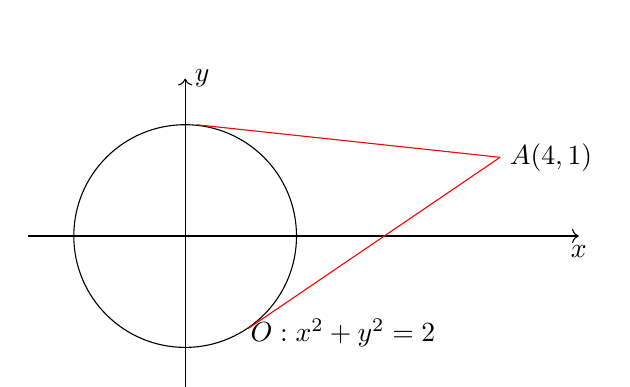
\begin{tikzpicture}
\coordinate [label=right:{$A(4,1)$}] (A) at (4,1);

\clip (-2,-2) rectangle (5.2,2.2);
\draw[->] (0,-2) -- (0,2) node[anchor=west] {$y$};
\draw[->] (-2,0) -- (5,0) node[anchor=north] {$x$};

% we must use node here for tangent coordinate system to work.
\node[circle, draw] (O) at (0,0) [inner sep=0, minimum size=2.82843cm] {};

\draw[color=red] (A) -- (tangent cs:node=O, point={(A)}, solution=1);
\draw[color=red] (A) -- (tangent cs:node=O, point={(A)}, solution=2);

\node[anchor=west] at (-60:1.414cm) {$O: x^2 + y^2 = 2$};

\end{tikzpicture}
\end{center}
\caption{构造圆与直线转化为斜率问题}
\label{flg:ConstructStraightLine}
\end{figure}

很易求出切线的斜率
\[
k = \frac{4 \pm \sqrt{30}}{14}
\]
故\(f(x)\)的最值分别为\(\frac{4 - \sqrt{30}}{14},\ \frac{4 + \sqrt{30}}{14}\).

\subsection{构造二项式}
一些关于求组合数的题目也挺有趣的,有些是构造二项式求解。比如:求
\[
\sum_{i=0}^n{\text{C}_{n}^i}
\]
便可通过构造\((1+x)^n\)并令\(x=1\)来求解。

然而课程中没有给上式,可能是觉得它太简单,转而给了一个这样的式子:
\[
\sigma = \sum_{i=0}^9{\text{C}_{10}^i\text{C}_{10}^{i+1}}
\]
在构造之前,先使用了组合数的性质把$\sigma$改写为
\[
\sigma = \sum_{i=0}^9{\text{C}_{10}^i\text{C}_{10}^{9-i}}
\]
这使得每一个乘积的上标之和都是9。随后构造\((x+1)^{10}(x+1)^{10}\),依二项式定理展开,得
\[
(\sum_{i=0}^{10}{\text{C}_{10}^ix^i})(\sum_{i=0}^{10}{\text{C}_{10}^ix^i})
\]
这让我们很易看出,在上标之和等于9得时候,$x$的次数也是9。而\(\sigma\)不是别的,正是\(x^9\)的系
数。现在把\((x+1)^{10}(x+1)^{10}\)合并为\((x+1)^{20}\),并求其中\(x^9\)的系数就是
\(\sigma\)了。显然,这系数是\(\text{C}_{20}^9\).

\section{课程:数学思想方法 -- 4 转化}
吐槽下,网课里说是转化与化归,竟然好多是转化成特殊值\footnote{这里的特殊值的意思是,不严谨的特殊
值,比如符合这个条件的情况中只取了一种,用这一种情况解答。}做的,我们不喜欢这样,我们觉得这样不是在做数
学,只是为了得分。既然你这样做,那我们就用超纲知识解了,请看网课里这道题:

设函数\(f(x) = \ln{x} + \frac{m}{x},\ m \in \mathbb{R}\),若
\[
\forall b > a > 0,\ \frac{f(b) - f(a)}{b - a} < 1
\]
恒成立,则$m$的取值范围是?

\textbf{解}:
显然$f(x)$在$[a,b]$上连续,$(a,b)$上可微,
依拉格朗日中值定理,
\begin{equation}
\frac{f(b) - f(a)}{b - a} = f'(c),\ c \in (a,b)
\end{equation}
另外,由于$f'(x)$也是连续的($x>0$),这使得对任意定义域上的$t$,可找到这样的
$b > a > 0,\ t \in (a, b)$,使得
$f'(t)$与$\frac{f(b) - f(a)}{b - a}$任意接近。
上面的讨论是在说明
\begin{itemize}
\item 对$\forall b > a > 0$,都可找到$c>0$,使$\frac{f(b) - f(a)}{b - a}$与$f'(c)$任意
接近(我们得到的是更严格的相等)。
\item 对$\forall c>0$,都能找到$b > a > 0$,使$\frac{f(b) - f(a)}{b - a}$与$f'(c)$任意
接近。
\end{itemize}
于是很易看出$f'(x)$的确界(如果有)与$\frac{f(b) - f(a)}{b - a}$的确界(如果有)相等。
而
\begin{equation}
f'(x) = \frac{1}{x} - \frac{m}{x^2}
\end{equation}
有上确界$\frac{1}{4m}$当$m > 0$时,于是$\frac{f(b) - f(a)}{b - a}$的上确界也是这个。
现在考察它能不能达到这个。事实上,这是不可能的,因为对某个
$\frac{f(b) - f(a)}{b - a} = f'(c)$,总能找到
\begin{equation}
f'(c') > f'(c),\ \frac{f(b') - f(a')}{b' - a'} = f'(c')
\end{equation}
于是接下来只要让$\frac{1}{4m} \leq 1,\ m > 0$就好了。

\subsection{转化为裂项相消}
这里说一下一个不是网课内容里的东西。
对形如$(an + b)c^n$的数列的求和,我们往往使用错位相减法。然而,在还未放假的时候,我们的数学老师转
而介绍了这样一种方法:用裂项相消求和。首先我们想一下裂项相消的条件。
首先要求$\sum_{i=1}^{n}{a_n}$的话,裂项一般是把$a_n$裂成$b_{n+1} - b_n$的形式。
这样$a_n + a_{n+1}$就能消去$b_{n+1}$。
于是问题就成为了求$b_n$使$(an + b)c^n = b_{n+1} - b_n$。首先考虑的是,$b_n$是不是也可以被
写成$(an + b)c^n$的形式。原理上来看,这是可以的。如果令$b_n = (a'n + b')c'^n$,那么
\[
b_{n+1} - b_n = c'^n[a'(c'-1)n + c'a' + c'b' -b']
\]
令
\begin{equation}
\begin{cases}
c' = c\\
a'(c'-1) = a\\
c'a' + c'b' - b' = b
\end{cases}
\end{equation}
就得出了一个符合条件的$b_n$。可能还有其他符合条件的,不过我们这里不需要求出其它的,只要保证充分性
就足够了。

这样,
\begin{equation}
\sum_{i=1}^{n}{a_n} = b_{n+1} - {b_1}
\end{equation}

\section{课程:数学思想方法 -- 5 分类讨论}

\subsection{排列组合中的分类讨论}
课程里大部分的分类讨论没什么好说的...分类几乎是只要基础扎实就很易看出的。我们一般在分类讨论上遇到问
题最多的地方就是在排列组合题上。经过一段时间的思考,我们总结出了一种方法能比较稳定地确定做排列组合题
的正确性。

大多数排列组合题的要求都是从一个给定集合中按某种题目要求的\emph{选法},取出一些元素,按照一定的顺
序,把它们排列起来。如果把这样一种排列叫做一种\emph{情况},题目一般是让我们求所有情况的个数。然而
经常出现根据题目要求的选法很难直接求出个数,于是我们常常构建一个和题目\emph{等价}的选法,用这个选
法求情况的个数。然而我们发现,光要求这个选法和题目的选法等价还是不够的,这可能会导致求出的情况个数变
多。我们对于两个选法等价的定义是:
\begin{itemize}
\item 给定的选法1得出的每一种情况都可以通过选法2得出,且
\item 选法2得出的每一种情况都可以通过选法1得出
\end{itemize}
为什么在实际中会导致求出的情况个数变多呢?以及,最奇怪的问题是,为什么当求出的情况个数不同时,
为何只会变多不会变少呢?毕竟这个选法等价关系和顺序无关啊\footnote{选法A等价于选法B与选法B等价
于选法A没区别}。为了回答这两个问题,我们思考了挺长的一段时间才发现了如下问题:首先题目的选法很特殊,
一般是给出了情况的限制条件 --- 既是,定义了什么样的情况满足题目要求。然而我们想出的选法却一般有这
样的特点:先分类\footnote{这也是为什么我们把这一部分放到分类讨论里面的原因。},再在每个分出的类别下
按某种选法选出满足题目要求的情况。这导致了可能出现在不同的分类下的选法选出了一样的情况,然而这并不
和选法等价冲突;而另一方面,题目给出的定义式选法不可能导致这种后果(或者说,定义本身就使得确定情况的
唯一性是我们的责任而不是题目的)于是这导致了我们的问题。

意识到这两个问题和它们的诱因后,我们又在想出的选法后加了一个条件,不仅要和题目选法等价,还要保证选出
的情况是唯一的,即不可能在两种不同的情况下,使用该选法选出同样的情况。或者即使该选法出现了重复的情
况,也可以很易通过一些方式在情况的数目中去掉它们。

让我们来看一些例子:

网课中的一道题是这样的:
有8张卡片分别标有数字$1,2,\cdots,8$,今从中取出6张排成3行2列,且只有第二行的两张卡片数字之和为
5,则不同的排法有?种?

很易看出这题目给了我们满足条件的情况的定义,让我们求情况数。现在我们来找一种选法。找到的选法为:
\begin{enumerate}
\item 先根据第二行的两张卡片数字之和为5,得出第二行要么是1,4要么是2,3,这情况有
$2! \times 2 = 4$种,
\item 之后我们有6张卡片要被填进4个空里,然而这里绝不是选4个填进去这么简单,因为题目中的``只有''
暗示了我们如果如果第二行是1,4,2,3就不能在另一行出现,反过来也一样。于是我们这里再分一次类,不妨以
第二行是2,3为例。则分1,4都被用到;1,4中只有一个被用到;1,4 \\
都没有被用到这3种情况。
\item 当1,4都被用到时,它们不能在一行。可以从所有求得的结果中删去它们在一行的结果,这做法比较好
理解。于是先从剩的4个数5,6,7,8中选2个出来有\(\text{C}_4^2=6\)种结果,之后得到了要用的4个数做
全排列 \\ 
\(4!=24\),再删去1,4在一行的情况\(2! \times 2! \times 2 = 8\),其中一个\(2!\)是1,4
的行排列,另一个是另外两个数的行的排列,最后的2是行上下颠倒。即选出的4个数的情况只有
\(24 - 8 = 16\)种。一乘得到\(16 \times 6 = 96\)种,
\item 当1,4中只有一个被用到时,从剩的4个数中选3个有\(\text{C}_4^3=4\)种,再对4\\
个数做全排列,然后一乘得\(24 \times 4 = 96\)种,再$\times 2$(因为1,4各一次)得结果192,
\item 当1,4一个都没有被用到时,直接做全排列\(4!=24\)就是最后的结果。
\end{enumerate}

现在我们考察这选法是否满足我们的要求。
首先证明它和题目的选法等价。首先题目得出的每一种情况都能被这选法得出,因为我们第一分类包含了所有的
情况,第二分类里面的情况都被排列/组合完全包含了。然后我们这选法得出的每一种情况显然都符合题目。

下面来看它是否能使选出的情况唯一。这是比较明显的。因为首先我们分的情况是互斥的,比如当1,4都被用到
时就不可能是1,4中只有一个被用到。然后在各个情况之中,排列/组合保证了得出情况的唯一性。

于是根据这选法来求情况数,是\(4 \times (24+192+96) = 1248\)种。

在这个考察过程中,发现了两点,第一:排列组合使各个分类下的细节计算得出情况的唯一性被保证,我们这里详
细提及,以后用到只要心里记得就好了。第二:如果分类是互斥的,分类的情况的唯一性就变得显然了,但这可能
并不会使问题更简单,因为有时我们改变分类使分类唯一时分类里面会变得复杂,这样本质上我们并没有消灭问
题而是把它推到了下一层,应该根据具体情况来定怎么分类。

\section{课程:数学思想方法 -- 6 放缩}
一些放缩用到的知识都比较基础,比如在分式中放大/缩小分母,在和式中放大/缩小每一项。这些的原理没什么
好说的,不过在应用中往往需要大量的尝试和经验来明白放缩到什么地步,这就很难能被总结出来。

在这一节,我们转而记载一些不是网课上,而是一些很经典的运用放缩法的证明,希望我们能从这些例子中总结出
一些有用的东西。

\subsection{伯努利不等式}
我们来看一下一个数学中很有名的被以\emph{Jacob Bernoulli}之名命名的伯努利不等式。
\subsubsection{严格形式证明}
伯努利不等式的严格形式\footnote{严格形式意味着严格的不等号(没有等号)}
是讲对一切整数$r \geq 2$,实数$x > -1,\ x \neq 0$,有
\begin{equation}
(1 + x)^r > 1 + rx
\end{equation}
它的证明本身也用到了一些放缩法。

\begin{proof}
把不等式左边依二项式定理展开,我们有
\begin{equation}
(1 + x)^r = 1 + rx + \cdots
\end{equation}
由于未写出的都是正的,这样当$x > 0$时不等式成立。

现在考察$-1 < x < 0$时。做替换$t=-x$,则$0 < t < 1$,
那么要被证明的成为
\[
(1 - t)^r > 1 - rt
\]
下面的证明就有一些技巧,请注意看:
\begin{align}
r 
&= \underbrace{1 + 1 + \cdots + 1}_{r\text{个}} \nonumber \\
&> 1 + (1-t)^1 + \cdots + (1-t)^{r-1} = \frac{1 - (1-t)^r}{1 - (1 - t)}
\end{align}
即是
\[
r > \frac{1 - (1-t)^r}{t}
\]
运用不等式的基本性质整理,就得到了我们想要的结果。
\end{proof}

\subsubsection{不严格形式证明}
接下来我们使用数学归纳法从另一个角度证明其不严格形式 (这里整数$r \geq 0$,实数$x \geq -2$):
\[
(1 + x)^r \geq 1 + rx
\]

\begin{proof}
首先我们证明对$r \in \{0,1\}$时不等式成立,之后证明如果对某个$r = k$已成立,则对$k + 2$也成
立,这样数学归纳法原理就能保证我们的命题成立了。

当$r = 0$时,显然,
\[
(1+x)^0 = 1 = 1 + 0x
\],不等式已成立。
当$r = 1$时,显然,
\[
(1+x)^1 = 1 + x = 1 + 1x
\],不等式已成立。

现在假设不等式对某个$r = k,\ k \geq 0$已成立,则
\begin{align}
(1+x)^{k+2} 
&= (1+x)^k(1+x)^2 \nonumber \\
&\geq (1+kx)(1+x)^2 \ \text{这里运用了不等式成立和}(1+x)^2\geq 0\text{的事实}
\nonumber \\
&= 1 + 2x + x^2 + kx + 2kx^2 + kx^3  \nonumber \\
&= 1 + (k+2)x + x^2(1 + k(x+2)) \nonumber \\
&\geq 1 + (k+2)x
\end{align}
数学归纳法原理保证我们的命题成立。
\end{proof}

\subsection{关于某个知名式子的放缩}
下面我们考察一个有名的式子,数列
\[
x_n = (1 + \frac{1}{n})^n
\]
在这一小节,我们将尝试放缩证明它的单调性和(上)有界性。

\begin{proof}
先证单调性,依二项式定理展开,
\begin{align}
x_n 
&= \sum_{i = 0}^{n}{\text{C}_{n}^{i}\frac{1}{n^i}} \nonumber \\
&= 1 + n\frac{1}{n} + 
\sum_{i=2}^n{\frac{n!}{i!(n-i)!}\frac{1}{n^i}} \nonumber \\
&= 2 + \sum_{i=2}^n{\frac{n(n-1)\cdots(n-i+1)}{i!}\frac{1}{n^i}}
\end{align}
注意到和式里面的$\text{C}_{n}^{i}$展开后的分式上面是$(n-0)$乘到$(n-(i-1))$共$i$项,
而$\frac{1}{n^i}$可以看成$i$个$\frac{1}{n}$相乘,故继续把$x_n$写成
\begin{align}
x_n 
&= 2 + \sum_{i=2}^n{\frac{1}{i!}\prod_{j=0}^{i-1}{\frac{n-j}{n}}} \nonumber \\
&= 2 + \sum_{i=2}^n{\frac{1}{i!}\prod_{j=0}^{i-1}{(1-\frac{j}{n})}}
\end{align}
\footnote{$\prod_{j=0}^{i-1}{f(j)}$的意思是$f(j)$从$j=0$乘到$j=i-1$,和和式$\sum $
表达形式差不多,以后我们把它叫做乘式。}
现在比较$x_{n+1}$与$x_n$的大小,我们发现在上式中把$n$变为$n+1$后,首先,和式又	多了一项,而这项
显然是正的;其次,在和式里已有的项中,乘式中的分母由$n$变为了$n+1$,然而这分式前面是$-$号,于是
整个式子变大。这就证明了$x_n$是递增的。

现在证明它上有界。很易看出,和式里面的乘式小于1。把它换成1使整个式子变大了一些,即
\[
x_n < 2 + \sum_{i=2}^n{\frac{1}{i!}}
\]
而在$i \geq 2$时,
\begin{align*}
\frac{1}{i!} 
&= \frac{1}{1 \times 2 \times \cdots \times i} \\
&< \frac{1}{1 \times \underbrace{2 \times \cdots \times 2}_{i-1\text{个}}} 
= \frac{1}{2^{i-1}}
\end{align*}
即
\[
x_n < 2 + \sum_{i=2}^n{\frac{1}{2^{i-1}}}
\]
又
\[
\sum_{i=2}^n{\frac{1}{2^{i-1}}} < 1
\]

则很易看出$x_n < 3$。
这就完成了证明。
\end{proof}

证明完后,我们额外地说一下它的重要性。由于$x_n$递增而又
上有界,于是它有一个有穷极限。这极限,不是别的,数学家\emph{Leonhard Euler}(欧拉)把它记为$e$。虽
然,这式子的极限最早不是欧拉,而是伯努利研究的,但伯努利当时并未指出这就是$e$。而数$e$本身,在更早
之前,被数学家\emph{John Napier}(纳皮尔)在他的关于对数的著作中提到过,不过当时他并未求出这是什
么。数$e$和$0,1,\pi,i$一样,在数学中起着重要的作用。它不仅作为自然对数的底,而且在很多领域都可能
甚至意想不到地出现。

\section{用导数证明不等式}
\subsection{用导数证明不等式的原理}
用导数证明不等式原理上比较简单。

\subsubsection{用导数与单调性的关系证明不等式}
我们知道,函数在某区间上(在区间内可导)具有(严格)单调性的一个必要且充分的条件是:
\begin{enumerate}
\item \emph{在区间内$f'(x)\geq 0$}
\item \emph{$f'(x)$不在任意区间上恒等于$0$}
\end{enumerate}
,注意我们说的是函数在某区间上有定义,但只需要它在区间内可导并且导数满足这些条件就好。
严格的证明在中学阶段还无法被做到,但这不影响这一事实在考试中被大量的应用。

那么给出函数$f(x)$在某区间上有定义且可导,之后对该区间上某点$x_0$\\
有$\forall x > x_0$,$f'(x) >(<) 0$,或者只有在不连续的点上$f'(x)=0$,
我们就有$f(x) > f(x_0)$对$\forall x >(<) x_0$。

事实上,甚至只要给定$f'(x_0) >(<) 0$就可以得到在$x_0$的足够小的邻域
\footnote{对某个点$c$,给定任意的$\delta > 0$,$(c-\delta,c+\delta)$就是它的一个邻域。}
上有这样的结论。这事实以后还要用到,我们先提一下。

这种证明不等式的方法需要的计算量比较小,只需求导,判断正负,最后
求临界处的$f(x)$值便好,很多题目中我们需要采取下一小小节的方法。

\subsubsection{用导数与函数极值点的关系证明不等式}
或者用到这样的方法证明不等式:用导数判断某函数在某区间上的最值,并发现这最值都比某个数大/小,
就得到了一个不等式。要采用这种方法,就要明白导数与函数极值点的关系。

对于极值点与导数零点的关系,很多地方说的不清楚,仅仅是指出``函数在某一点上存在极值并不是这一点导数
为0的必要且充分的条件''这样的事实。事实上,这两者的关系被费马定理确定了。另外,课本上也没有严格定义
极值点是个什么东西,这里说明一下。

{\em 如果在函数定义域内存在这样一个点$x_0$,使得在它的一个被包含在定义域内的邻域内,都有
$f(x) >(<) f(x_0)$那么$x_0$是函数$f(x)$的一个极小(大)值点。}

\textbf{费马定理}:
\emph{设函数在某一区间上有定义,且在该区间的内点$x_0$上有某个极值。那么,如果$f'(x_0)$存在,则
$f'(x_0)=0$.}

这意味着在某一点处取得极值与导数值为0既不是必要关系,也不是充分关系。

为了得到函数取得极值的更进一步的关系,我们还需要加更多的限制。下面我们将进一步考察函数的性质。

首先要被说明的是最值的存在性。如果函数$f(x)$在某个闭区间上有定义且可导,那么它在这个区间上就连续。
既然它在这个区间上连续,根据\textbf{魏尔斯特拉斯}(\emph{Karl T.~W.~Weierstrass})
\textbf{第二定理},它在这个区间上必能达到最大值和最小值。
魏尔斯特拉斯第二定理是怎么来的我们暂时不需要知道,只需要知道函数最值存在的事实就好了。

既然最值存在,我们只要找到这函数所有的极值点,最值点就在它们之中了(注意区间两端点也可能是极值点)。

首先既然函数已经可导了,那么根据费马定理,$f'(x)=0$就成为了极值点存在的必要条件。下面我们来看充分
条件是个什么东西。首先对所有$f'(x)=0$的点,极值点一定在他们里面,我们现在筛选就可以了。如果至少在
这样的一点的一个邻域中,$f'(x)$在两边分别保持着不同的符号,那么这个点就是一个极值点,极大值和极小
值由两边符号决定,如果左边$-$右边$+$,那么就是极小值,反过来,就是极大值。证明是很易被看出的。

然而现实情况中,导函数在两边的符号情况难以被直接看出,这就使我们不得不寻找别的方法来确定符号。我们
可以考虑求二阶导数。根据我们在上一个小小节提到的那个事实,假定二阶导数在这个点处不是0,我们的条件
就被满足了。$f''(x)>0$时,这个点是极小值,反之,是极大值。

然而可能遇到这种情况,二阶导数在这一点上也是0,或者更糟,不仅是二阶导数,一直到$n$阶导数在这一点上
都是0。在这里,我们不加证明地给出如下结论(因为现阶段无法证明):

\emph{若第一个不为$0$的导数是奇数阶的(比如$1$阶导数,$3$阶导数),函数在这一点没有极值,如果是偶
数阶的,则有极值,如果这第一个不为$0$的偶数阶导数在这是正的,则是极小值,是负的就是极大值。}

即使是这样,也可能遇到在某函数的一点处任意阶导数为0。在这情况下是没有一般的法则判断的,因为能够
找出函数使得在一点处一切阶导数为0但这点不是极值点,同时也能找出函数使得在一点处一切阶导数为0但这
点是极值点。

\subsection{例子}
让我们来看一些例子:

(1) 求证$x \in (0,\frac{\pi}{2})$时$x < \tan{x}$.
\begin{proof}
首先,$x=0$时,$x=\tan{x}$。其次,
\[
\tan'{x} = \frac{1}{\cos^2{x}} \geq x' = 1
\],
就完成了证明。
\end{proof}

(2) 下面我们来看这个例子,我们用两种方法证明。
求证$x \in (0,\frac{\pi}{2})$时\\
$\sin{x} > \frac{2}{\pi}x$.

第一种方法
\begin{proof}
首先,$x=\frac{\pi}{2}$时,$\sin{x}=\frac{2}{\pi}x$。其次,
\[
\sin'{x} = \cos{x} > \frac{2}{\pi}
\]
直到某个值使$\cos{x} = \frac{2}{\pi}$。这意味着$\sin{x}$最可能小于$\frac{2}{\pi}x$的地方
是$\frac{\pi}{2}$,虽然取不到,但可以取极限,发现正好相等,就完成了证明。 \qedhere

这证明和用导数判断极值本质上没什么区别。
\end{proof}

第二种方法:
\begin{proof}
在这方法里,我们用单调性来证明,然而就像上一种方法里提到过的,这两者导数并不总是一个比另一个大,
于是我们尝试构造新函数\\
$\varphi(x) = \frac{\sin{x}}{x}$,注意这里$\varphi(x)$的定义域我们
把$\frac{\pi}{2}$加上为了后面方便。
而
\begin{equation}
\varphi'(x) = \frac{\cos{x}(x-\tan{x})}{x^2}\ (0 < x < \frac{\pi}{2})
\end{equation}
由于我们在(1)中证明的$x \in (0,\frac{\pi}{2})$时$x < \tan{x}$,
这导致了$\varphi'(x)$总是负的在$(0 < x < \frac{\pi}{2})$时,于是
$\varphi(x)$在$(0,\frac{\pi}{2}]$上都是严格递减的,故
\[
\varphi(x) > \varphi(\frac{\pi}{2}) = \frac{2}{\pi}
\]
运用不等式的基本性质整理便得到了我们的结果。
\end{proof}

(3) 我们考察函数
\[
f(x) = x^a - ax\ (0 < a < 1),(x \geq 0)
\]
。我们有
\[
f'(x) = a(x^{a-1}-1)
\begin{cases}
> 0\ (0< x <1)\\
< 0\ (x>1)
\end{cases}
\]
于是$f(x)$有最大值$f(1)$
这意味着
\begin{equation}
x^a - ax \leq 1 - a
\end{equation}

我们可以从这个不等式推出一个我们很熟悉的不等式。
首先令$x=\frac{\alpha}{\beta},\alpha,\beta>0$,
然后令$1-a=b$,于是原不等式可被写成
\[
\alpha^a\beta^b \leq a\alpha + b\beta
\],
$a,b,\alpha,\beta > 0,\ a + b = 1$.
之后引入正数$p,q>0$,令$a=\frac{p}{p+q},b=\frac{q}{p+q}$。
我们有
\[
(\alpha^p\beta^q)^\frac{1}{p+q} \leq \frac{p\alpha + q\beta}{p+q}
\]
令$p=q=1$,我们得到了十分熟悉的老朋友
\begin{equation}
\sqrt{\alpha\beta} \leq \frac{\alpha + \beta}{2}
\end{equation}

\section{经典例题}
让我们来看看一些经典例题。

\subsection{2019 -- 2020烟台期末T22}
考虑函数
\[f(x) = (\frac{1}{2}x^2 - ax)\ln{x} + 2ax - \frac{3}{4}x^2\], 
其中\(0 < a < e\).

\begin{enumerate}
\item 求函数\(f(x)\)的单调区间;
\item 讨论\(f(x)\)的零点个数;
\item 若\(f(x)\)存在两个不同的零点\(x_1,\ x_2\),  求证\(x_1x_2 < e^2\).
\end{enumerate}
\textbf{解}:

\subsubsection{(1)}
很易求出
\begin{align}
f'(x) 
&= (x - a)\ln{x} + \frac{1}{2}x - a + 2a - \frac{3}{2}x \nonumber \\
&= (x - a)\ln{x} - x + a \nonumber \\
&= (x - a)(\ln{x} -1)
\end{align}

当\(0 < a < e\)时, 
\begin{center}
\begin{tabular}{|c|c|c|c|c|c|}
\hline
\(x\) & \((0,\ a)\) & \(a\) & \((a,\ e)\) & \(e\) 
& \((e,\ +\infty)\) \\
\hline
\(f'(x)\) & \(+\) & 0 & \(-\) & \(0\) & \(+\) \\
\hline
\(f(x)\) & \(\nearrow\) & 极大 & \(\searrow\) & 极小 & \(\nearrow\) \\
\hline
\end{tabular}
\end{center}

单调区间就很易看出了。

\subsubsection{(2)}
首先考察两端的趋势。\footnote{这里用到了一些越出了高中数学范围的极限的基本知识,然而高中数学
对这一方面的态度十分暧昧,很多既要用到却不在学习的范围内,只能老师补充或自学,所以我们就用了。}
然而\(\lim_{x \rightarrow 0^{+}}{(\frac{1}{2}x^2 - ax)\ln{x}}\)比较难求。
首先证明:
\[
\lim_{x \rightarrow 0^{+}}{-ax\ln{x}} = 0
\]
\begin{proof}
要证这一点,只需做替换\(t=\frac{1}{x}\)得
\begin{align}
\lim_{x \rightarrow 0^{+}}{-ax\ln{x}} 
&= \lim_{t \rightarrow +\infty}{-a \cdot \frac{1}{t}\ln{\frac{1}{t}}} 
\nonumber \\
&= \lim_{t \rightarrow +\infty}{\frac{a\ln{t}}{t}} \nonumber \\
&= 0 \qedhere
\end{align}
\end{proof}

所以显然\(\lim_{x \rightarrow 0^{+}}{\frac{1}{2}x^2\ln{x}} = 0\)
于是
\begin{equation}
\lim_{x \rightarrow 0^+}{f(x)} = 0
\end{equation}.

而\(\frac{1}{2}x^2\ln{x}\)在\(x \rightarrow +\infty\)时是比\(\frac{3}{4}x^2\)更高阶
的无穷大,故
\begin{equation}
\lim_{x \rightarrow +\infty}{f(x)} = +\infty
\end{equation}

当\(0 < a < e\)时,有没有零点取决于\(f(e)\)的值。
\begin{align*}
f(e) 
&= -\frac{e^2}{4} + ae\\
&= e(-\frac{e}{4} + a)
\end{align*}
当\(a > \frac{e}{4}\)时,没有零点;\(a = \frac{e}{4}\)时有一个;
\(a < \frac{e}{4}\)时有两个。

\subsubsection{(3)}
这时\(0 < a < \frac{e}{4}\)
有一个简单的做法。
图\ref{fig:dfdx} 展示了\(f(x)\)当
\(a=\frac{e}{8}\)时的图像。

\begin{figure}[!htbp]
\begin{center}
\begin{tikzpicture}
\begin{axis}[
axis lines=center,
title={$a=\frac{e}{8},\ x \in (0.5,5),\ f(x)$},
xlabel={$x$},
ylabel={$y$},
xmin=0.5, xmax=5,
]
\addplot[black,samples=201] 
{(0.5*x*x-0.125*e*x)*ln(x)+0.25*e*x-0.75*x*x};
\end{axis}
\end{tikzpicture}
\end{center}
\caption{\(f(x) = (\frac{1}{2}x^2 - ax)\ln{x} + 2ax - \frac{3}{4}x^2\)}
\label{fig:dfdx}
\end{figure}

\begin{proof}
考虑
\begin{align}
f''(x)
&= \ln{x} + 1 - \frac{a}{x} - 1 \nonumber \\
&= \ln{x} - \frac{a}{x} 
\end{align}
以及
\begin{equation}
f'''(x) = \frac{1}{x} + \frac{a}{x^2}
\end{equation}
\begin{align*}
&\because \forall x \in (c, +\infty), f'''(x) > 0\\
&\therefore \forall x_1, x_2\ (x_1>x_2) \in (c, +\infty), f''(x_1) > f''(x_2)\\
&\therefore \forall t < e - c, f''(e-t) < f''(e+t)\\
\text{又} &\because \forall x \in (c, +\infty), f''(x) > 0, f'(e) = 0\\
&\therefore \forall t < e - c, |f'(e-t)| < |f'(e+t)|
\end{align*},其中\(f''(c)=0\)。
最后一步推理比较显然,因为\(f'(x)\)在\(e\)右侧比左侧增地快。不过这不怎么严谨。严格地
证明的话可以构造一个新函数把右侧的\(f'(x)\)与左边的翻转后相加,比如令
\(\varphi (x) = f'(e+x) + f'(e-x)\),易得\(\varphi '(x) > 0\),详细过程就不写了。
这样,\(f(x)\)在两零点间的极值点右侧比左侧增的快,这意味着设\(x_1, x_2\ (x_2 > x_1)\)为两零
点,有\(x_2 - e < e - x_1\),故
\begin{equation*}
x_1x_2 < [e + (x_2 - e)][e - (x_2 - e)]
< e^2 \qedhere
\end{equation*}
\end{proof}

寒假数学到这里就结束了,网课里还有一些剩下的内容,不过我不打算写了,我要去做题了。

\newpage
\part{Winter Vacation English: How to Write DuHouXuXie}
\begin{quotation}
{\ttfamily ``We tell ourselves stories in order to live...

\begin{sloppypar}
We look for the sermon in the suicide, for the social or moral lesson in the 
murder of five. We interpret what we see, select the most workable of the 
multiple choices. We live entirely, especially if we are writers, by the 
imposition of narrative line upon disparate images, by the "ideas" with which we 
have learned to freeze the shifting phantasmagoria which is our actual 
experience.''
\end{sloppypar}
--- Joan Didion\cite{TellStoriesToLive}

``The purpose of a storyteller is not to tell \\
you how to think, but to give you 
questions to think \\
upon.''

--- Brandon Sanderson}
\end{quotation}

\newcommand{\GK}{GaoKao}
\newcommand{\DHXX}{DuHouXuXie}
\newcommand{\TriActStruct}{Three-act structure}

Writing has become more important in GaoKao recently as \DHXX{} has been added.
\DHXX{} is essentially to continue small story, so it has the qualities of a 
story. On the other hand, it is so small many aspects are restricted. In this 
part, 
we will focus on the features of \DHXX , and introduce some skills as well.

\section{Features of \DHXX}
A typical story includes several main characters, as well as their relationships,
characteristics and the world they live in. These components are usually 
introduced at the very beginning of a story. In \DHXX , the beginning is already 
given.

The \DHXX{} is rather short. We need to finish the story in about 200 words and 
this could be a challange to the development of the story. We have no time and 
space to comprehensively describe everything but to concentrate on the story and 
characters. 

As for the type of the story, things that are considered not suitable for 
students by the Chinese society, for example, romantic love, are not recommended 
to be conveyed in the story, despite the fact that most of them are highly 
effective at drawing readers attentions and are of the types of the most famous 
novels.\footnote{Affections to these things are natural to human beings, and I 
have always wonder why there is merely a country like China that uses the word 
``ZaoLian'' to show disapproval to romantic love of adolescents.}

\section{How to Write a Good Story}

\subsection{Model and Structure}
We can decide what structure to use in our story but the effect may not be good. 
It is better to use some model that is already successful and effective to struct 
our story, because we don't have much time to pratice our own model. 

\subsubsection{The \TriActStruct{} Model}
There is a classic model called the ``\TriActStruct '' that is used in narrative 
fiction.\footnote{We will only introduce its basic concepts, for more 
information, see\cite{TriActStruct}}

The \TriActStruct{} divides a story into three parts (acts) --- the Setup, the 
Confrontation, and the Resolution. The Setup establishes main characters, 
introduces their relationships and presents the world they live in. Then somehow 
an incident called the first turning point occurs, and the attemps to deal with 
the incident lead to the first plot point. Contents before the first plot point 
are often included in the given story, so what we need to do on the Setup part is 
to give our own first plot point. The first plot point generally does three 
things:
\begin{enumerate}
\item signals the end of the first act,
\item ensures life will never be the same again for the protagonist and
\item raises a dramatic question that will be answered in the climax of the 
story.
\end{enumerate}

Then the confrontation begins and our story goes around the problem initiated by 
the first turning point. The protagonists try to resolve the problem, and the 
following problems are described. Characters are developed in this act, but 
note that their characteristics may be implied in the given story. Along the way 
of trying to resolve the problem, the protagonists gradually realizes who they 
are, and the attempts to resolve the problem unexpectedly changes who they are.

Eventually the problems are resolved and the climax, where the main tensions of 
the story are brought to their most intense point and the dramatic question 
answered, leaving the protagonist and other characters with a new sense of who 
they really are.

The structure of our story can be slightly different from the \TriActStruct . We 
don't need to fit in the format exactly, and we don't have to use only one 
structure.

Let's consider an example:

\begin{quotation}
{
\sffamily
It was summer, and my dad wanted to treat me to a vacation like never before. He 
decided to take me on a trip to the Wild West.

We took a plane to Albuquerque, a big city in the state of New Mexico. We reached 
Albuquerque in the late afternoon. Uncle Paul, my dad's friend, picked us up from 
the airport and drove us up to his farm in Pecos.

His wife Tina cooked us a delicious dinner and we got to know his sons Ryan and 
Kyle. My dad and I spent the night in the guestroom of the farm house listening 
to the frogs and water rolling down the river nearby. Very early in the morning, 
Uncle Paul woke us up to have breakfast. ``The day starts at dawn on my farm,'' 
he said. After breakfast, I went to help Aunt Tina feed the chickens, while my 
dad went with Uncle Paul to take the sheep out to graze. \textcolor{blue}{I was 
impressed to see my dad and Uncle Paul riding horses. They looked really cool.}

\textcolor{blue}{In the afternoon, I asked Uncle Paul if I could take a horse 
ride, and he said yes, as long as my dad went with me. I wasn't going to take a 
horse ride by myself anyway. So, my dad and I put on our new cowboy hats, got on 
our horses, and headed slowly towards the mountains.} ``Don't be late for 
supper,'' Uncle Paul cried, ``and keep to the track so that you don't get lost!'' 
``OK!'' my dad cried back. After a while Uncle Paul and his farm house were out 
of sight. It was so peaceful and quiet and the colors of the brown rocks, the 
deep green pine trees, and the late afternoon sun mixed to create a magic scene. 
It looked like a beautiful woven blanket spread out upon the ground just for us. 

\paragraph{Paragraph 1} 
\textcolor{red}{Suddenly a little rabbit jumped out in front of my horse.}

\paragraph{Paragraph 2}
\textcolor{green}{We had no idea where we were and it was getting dark.}
}\\
\begin{large}
\textbf{Possible Version:}
\end{large}

{
\sffamily
\paragraph{Paragraph 1}
\textcolor{red}{Suddenly a little rabbit jumped out in front of my horse. Dad and 
I found it was so cute that we decided to chase it. After a while, we were 
completely lost in the forest.} There was nothing left in our sight but the 
trees. ``We may not be able to make it back to the farm house in time for 
supper.'' I thought to myself. \textcolor{green}{After a series of fruitless 
attempts to find a way out, we felt hungry and tired.}

\paragraph{Paragraph 2}
\textcolor{green}{We had no idea where we were and it was getting dark. We got 
stuck in the forest. And an unexpected shower added to the difficulty of us in 
finding a way home, for all the tracks we had made disappeared because of the 
rain.} \textcolor{orange}{I was almost on the edge of breaking down when my 
father said, ``Don't worry, my son. I remember there is a river near the farm 
house. Find the river and we will be back home.''} Finally, we found the river 
and got back to the house along it. Needless to say, we ate a late dinner.}
\\
--- GaoKao ZheJiang, 2019
\end{quotation}

The text colored with \textcolor{blue}{blue} is the \textcolor{blue}{first 
turning point}; the text colored with \textcolor{red}{red} is the \textcolor{red}
{first plot point}; the text colored with \textcolor{green}{green} is the 
\textcolor{green}{difficulties and problems the protagonists met while trying to 
solve the problem.}; and the text colored with \textcolor{orange}{orange} is the 
\textcolor{orange}{climax} of the story.

As we can see, there are some differences between the story and the \TriActStruct 
. For example, the main characters' live has not been changed after the climax. 
It is another example that the we don't need to fit in the format exactly. 
Furthermore, the possible version is such a tight story that there is hardly
something that develops the characters.

This successful structure ensures that \emph{provided you follow this sturcture, 
your story will be attrative}. The result is quiet stable, but some people don't 
like making stories this way. They might want to develop their own structures, 
which is also a possible way, though it can be more difficult. We won't describe 
this way in this note. Further reading can be found at \cite{StoryStructure}, 
where Steph Fraser tells us how to create a novel structure and some available 
structures.

\subsection{Conversation and Dialogue}
Conversation is of vital importance in most stories, so we use a subsection to 
talk about it. 

\subsubsection{Rules}
There are some rules that are useful when writing dialogue. Do remeber, 
\textbf{DIALOGUE MUST BE THERE FOR A REASON}\@. In other words, dialogue must be 
meaningful to our story. In fact, some pointless dialogue is good in a novel, but 
\DHXX{} is a damn small story, so make sure you don't write pointless 
conversation.

The reasons why a dialogue is there can be:
\begin{itemize}
\item it attracts readers' attention, or
\item it advances the story, or
\item it deepens characters' personalities, or
\item it supplies information.
\end{itemize}

To draw readers' attention, the most common technique is to include 
\emph{conflicts} in conversation. The conflict can be the disagreement between 
several characters, or the contradiction between reality and fantasy. By using 
conflicts in dialogue, the story becomes intenser. This is different from our real 
life, in which we may spend weeks without exciting things. Here is an example:

\begin{quotation}
In this example, we have a dialogue between Estella and Pip in Charles Dickens'
\emph{Great Expectations}\cite{GreatExpect}, where Estella was insulting poor Pip.

{\sffamily 
``Well?'' \par
``Well, miss?'' I answered, almost falling over her and checking myself. \par
``Am I pretty?'' \par
``Yes; I think you are very pretty.'' \par
``Am I insulting?'' \par
``Not so much so as you were last time,'' said I. \par
``Not so much so?'' \par
``No.'' \par
She fired when she asked the last question, and she slapped my face with such 
force as she had, when I answered it. \par
``Now?'' said she. ``You little coarse monster, what do you think of me now?''
\par ``I shall not tell you.''
}
\end{quotation}

We can see the conflict between Estella and Pip, and we might be curious about 
the reason why Estella was so mean, which was finally turned out as a consequence 
of her breeding.

We can also provide questions in dialogue, especially yes or no questions like 
``Will the boy get that girl?''; ``Will the characters survive the disease?''. 
Questions make the story more dramatic.

Multiple ways are available to drive the story forward. It might increase the 
suspense for what is coming, give some hints to what the characters want, or 
change the situation the characters are in.

The following illustration shows a good conversation that advances the story from 
\emph{Gone With The Wind}\cite{GWTW}.

\begin{quotation}
{\sffamily
``Sir,'' she said, ``you are no gentleman!''

``An apt observation,'' he answered airily. ``And, you, Miss, are no lady.'' He
seemed to find her very amusing, for he laughed softly again. ``No one can remain
a lady after saying and doing what I have just overheard. However, ladies have
seldom held any charms for me. I know what they are thinking, but they never
have the courage or lack of breeding to say what they think. And that, in time,
becomes a bore. But you, my dear Miss O'Hara, are a girl of rare spirit, very 
admirable spirit, and I take off my hat to you. I fail to understand what charms 
the elegant Mr.~Wilkes can hold for a girl of your tempestuous nature. He should 
thank God on bended knee for a girl with your---how did he put it?---`passion for 
living,' but being a poor-spirited wretch ---''

``You aren't fit to wipe his boots!'' she shouted in rage.

``And you were going to hate him all your life!'' He sank down on the sofa and
she heard him laughing.
}
\end{quotation}

The remarks Rhett gave Scarlett such as  ``\emph{But you, my dear Miss O'Hara, are 
a girl of rare spirit, very admirable spirit, and I take off my hat to you.}'' 
shed some light to what might have happened to Rhett and Scarlett.

Dialogue can also further develop characters' personalities. However, as mentioned 
many times before, we probably haven't enought space for such dialogue to occur. 
Then comes the information providing, which is useful in writing \DHXX . Some 
backgrounds will seem more natural if we put them into dialogue.

\subsubsection{Tips}

In dialogue novels, each speaker gets their own paragraph, and the paragraphs are 
indented, which makes the dialogue clear and brief. In \DHXX , however, we don't 
have enough space, so we need to merge those paragraphs into one huge paragraph. 
As a consequence, it might become unclear about who is speaking, so please denote
the speaker when necessary.

To save space, we can add additional information at the end of dialogue. For 
example, 
\begin{quote}
``There, there, Mrs.~Meade'' said the doctor, basking obviously in the praise.
\end{quote}

Then avoid small talks in your dialogue. They might be useful in novels, but not 
here. And also, make the dialogue concise and brief. This not only because we have 
little space, but can also improves the dialogue quality.

You can cut out goodbyes and hellos to save space as well as to speed up your 
pace, as long as your readers understand the situation well.

Finally, try to give each speaker a unique voice, which greatly improves the 
story.

\subsection{Character Development}
We are probably not able to develop a character fully in \DHXX , but I will 
nevertheless introduce it here briefly, as a reason of its importance in 
literature.

The character development is not just to show a imaginary person to your readers, 
you need to show them how this person changes and transforms throughout the story. 
Is is the process of creating a person AS WELL AS the changes he goes through.

The characters are already given in the given story, but their personalities may 
not be decided yet. You can develop them on your own, but ensure that you have 
identified your characters and their roles. And when your try to develop them, 
think things in their situation --- What would you do if you were him?

Please refer to other resources for more information.

By now, our brief introduction about how to write a good \DHXX{} comes to an end.
There are still some aspects (e.g. environment) haven't been described yet, but 
they are less important than the things we described before in \DHXX due to its 
space limit. You can learn about them as much as you want in the future, and 
Best Wishes :) !

\newpage
\part{寒假物理:光学和量子力学初步}
\begin{quotation}
``自然是不是可能像在这些原子实验里的这样荒诞?''

{\ttfamily
\begin{sloppypar}
``Can nature possibly be so absurd as it seemed to us in these atomic 
experiments?''
\end{sloppypar}

--- Werner Heisenberg}

``物理就像性一样,它的确能带来一些有用的结果,但那不是我们为什么做它的原因。''

{\ttfamily
``Physics is like sex: sure, it may give some \\
practical results, but that's not why 
we do it.''

--- Richard Feynman}

\end{quotation}

\section{光学初步}
光学主要研究光的性质,现象及其应用。人类对于光的研究很早就开始了,随着人们对光认识和其它领域研究
的进步,光学逐步发展,到了现在,人们已经不得不用量子力学来解释光的一些行为了。

我们先来谈谈在历史上被大量研究的光学,几何光学。它试图将光看作一条射线,并能成功解释光的折射,反射
等一些现象。反射就不提了,早在初中我们都已接触过并认识了这方面的内容。

\subsection{光的折射}
先不谈网课上的内容,来看一个课本上的例子。课本上的光的折射定律大家应该很熟悉了,
它又被称为Snell定律,因为Snell (Willebrord Snellius)最先给出了它的一个数学关系式。
\[
\frac{\sin{\theta_1}}{\sin{\theta_1}} = \frac{v_1}{v_2} = \frac{n_1}{n_2}
\]
这个定律既可以被从费马原理\cite{FMsPrinciple}推导出来,也可以从我们课本上介绍的惠更斯原理被推
导出来\footnote{事实上它还可以从麦克斯韦方程组,或是从能量守恒和动量守恒,或是从平移对称性原理等
中被推导出来。然而这些推导无法被做到在中学阶段。}。

\subsubsection{用费马原理推导Snell定律}
我们先看一下用费马原理推导它。费马原理告诉我们,光线跑的路不是别的,而是用时最短的路。现在,如图
\ref{fig:DeriveSenllsLawFromFermats},
我们在线两侧有两个不同的介质区域$A, B$,其中分别存在点$P, Q$,现在有光要从$P$跑到$Q$,我们尝试
用费马原理找到它的路径。

\begin{figure}[!hbpt]
\begin{center}
\begin{tikzpicture}
\coordinate[label=left:{$P$}] (P) at (3,2);
\coordinate[label=right:{$Q$}] (Q) at (-2,-3);
\coordinate[label=above left:{$M$}] (M) at (0,0);

\node[anchor=west] at (0,1.5) {$A$};
\node[anchor=east] at (0,-1.5) {$B$};

\draw[very thick] (-4,0) -- (4,0);
\draw[dashed] (0,2.5) -- (0,-2.5);

\draw[->] (P) -- (1.5,1);
\draw (1.5,1) -- (M);
\draw[->] (M) -- (-1,-1.5);
\draw (-1,-1.5) -- (Q);

\end{tikzpicture}
\end{center}
\caption{用费马原理推导Snell定律}
\label{fig:DeriveSenllsLawFromFermats}
\end{figure}

\begin{proof}
首先证明,光在两个介质内跑的不是别的,而是直线。首先,光无论怎么跑,都要经过分界线上的某一点M,于是
连接$PM,PN$,显然,光跑别的路径要比它跑直线跑的更长,就得出了光要跑直线。得出路径后就好算时间了。
设$P,Q$到分界线的距离分别为$a,b$,它们之间的水平距离为$l$,设$M,P$间的水平距离为$x$,光在$A,B$
中的速度分别为$v_1,v_2$,
则时间
\begin{equation}
t = \frac{\sqrt{a^2 + x^2}}{v_1} + \frac{\sqrt{b^2 + (l-x)^2}}{v_1}
\end{equation}
求导
\begin{equation}
\frac{\mathrm{d}t}{\mathrm{d}x} = \frac{x}{v_1\sqrt{a^2 + x^2}} + 
\frac{-(l-x)}{v_2\sqrt{b^2 + (l-x)^2}}
\end{equation}
很易看出,导数零点就是极小值点。
注意到,
\begin{align*}
\frac{x}{v_1\sqrt{a^2 + x^2}} &= \sin{\theta_1} \\
\frac{(l-x)}{v_2\sqrt{b^2 + (l-x)^2}} &= \sin{\theta_2}
\end{align*}
,其中$\theta_1,\theta_2$分别是$PM,QM$与法线成的角。
这就完成了证明。
\end{proof}

用惠更斯原理推导这里就不讲了。

\subsubsection{折射率和全反射}
显然,当两边介质一样的时候,光在里面传播的速率也一样,那么这个折射角的正弦之比就是定值。我们把这个
比值记为$n$. 如果令$\theta_1$表示光在真空中的入射角,这时的$n$就被定义为某种介质的(绝对)折射
率。光的相对折射率就很好理解了,就是把一种介质的入射角作为$\theta_1$,这样$n$就成为了某介质相对
于该介质的折射率。

从上面的推导我们能看出,折射率也可用$\frac{v_1}{v_2}$即是速度的比值表示。因为光在空气中传播的速
度和在真空中传播的速度几乎相等,我们就可以认为,某种介质的绝对折射率就近似等于以空气中入射角为
$\theta_1$的$n$. 

我们可能会发现一个问题,首先,光在真空中跑得最快,所以$n$总是大于1的。而因为$n$总是大于1的,
$\theta_1,\theta_2$就不能跑遍$(0,\frac{\pi}{2})$之间的每一个值。准确地讲,因为
\begin{equation}
\sin{\theta_1} = n\sin{\theta_2}
\end{equation}
所以$\theta_2$只能在$(0,\arcsin{\frac{1}{n}})$里被取值。一旦它越出这个范围,$\theta_1$就成
为了未被定义的。为了研究这种情况下的折射是个什么情况,我们还需要重新做实验来看看。

这时做实验我们显然就不能通过变动$\theta_1$来做了,而是要变动$\theta_2$使它越出
$(0,\arcsin{\frac{1}{n}})$的范围。大量的实验表明,在这种情况下,折射完全丢失了,只剩下反射光。
我们把这种现象称为全反射。

这样,我们把发生全反射的临界角记作$C$,而
\begin{equation}
C = \arcsin{\frac{1}{n}}
\end{equation}

\subsubsection{光的色散和它与折射的关系}
据说是牛顿最先发现了这一现象---他把阳光透过三棱镜后,发现它变成了一条七种颜色的色带。

我们尝试用我们刚谈过的折射理论来研究这个问题。把阳光看成一道光从空气入射进入三棱镜(玻璃),然后再
出射,而最后出射的角度不一样。通过分析表明,这意味着折射率的不同。然而一束光怎么会有不同的折射率在
相同的介质里呢?人们经过探索和思考,认为这是因为阳光是多种色光的结合,而各种色光在玻璃的折射率不一
样。根据我们之前的公式,这暗示着不同颜色的光在相同介质中的传播速度可能不同。

在之后,我们会谈到光的波动性,事实上,光的波动性最先被提出不是因为别的,而是为了解释颜色的起源。
科学家胡克(Robert Hooke)开发了一个振动理论为了解释颜色的起源,并且他把光和水波的传播做了比较。
之后,惠更斯(Christiaan Huygens)做出了一个光的波动说的数学理论。

\subsection{光的波动性}
在人们研究光的过程中,发现了一些无法用几何光学来解释的事实。我们之前提过,惠更斯等人提出了波动说,
而与此对应,牛顿提出了微粒说,认为光是由一些特殊性质的微粒构成的。由于牛顿的权威性,在长达一个多世
纪的时间内,波动说一直都处于弱势,直到物理学家杨(Thomas Young)用实验证实了光具有波的重要性
质---这实验正是著名的双缝干涉实验。

\subsubsection{光的干涉}
在课本上,给出了一种推导两个亮/暗条纹之间距离$\Delta r$与
与双缝间距离$d$、挡板与屏距离$l$和光波长$\lambda$的近似公式
\begin{equation}
\Delta r = \frac{l}{d}\lambda
\end{equation}
该公式当$l$远大于$d$时近似成立。

我们知道,双缝干涉的原理是当屏上一点到两缝的距离差刚好是
光波长的整数倍时,两个相干波源发出的某个波峰就会同时到达那一点,叠加加强。事实上,不仅是双缝,只要是
能产生相干波源(即是,两个震动情况总是相同)的一些器械也能在某种限定下使我们观察到干涉现象。

另外,不仅仅是这样的相干波源,即使是跟某一个波源的震动相差一些相位的另一个波源,它们之间也能发生
干涉。比如薄膜干涉,来自前表面的反射光和来自后表面的反射光振动相差一些相位,如果它们到人眼的距离差
正好等于它们差的相位乘波长的话,就得到了加强光。

\subsubsection{光的衍射}
最早仔细观察衍射并对其命名的是意大利物理学家弗朗西斯科\\
(Francesco Maria Grimaldi)。他指出:
\begin{quote}
``光不仅会沿直线传播、折射和反射,还能够以第四种方式传播,即通过衍射的形式传播。''\\
``Lumen propagatur seu diffunditur non solum directe, refracte, ac 
reflexe, sed etiam alio quodam quarto modo, diffracte.''
\end{quote}
并把衍射命名为\emph{diffraction},从拉丁文的\emph{diffringere}里得到启发,意思是
``破碎成碎片'',来表示光的传播方向被打碎成不同的各种方向。

衍射是指的是波穿过障碍物后发生不同程度的弯曲传播。我们知道,日常生活中的光基本都是沿直线传播,
然而我们尝试用很小的孔让光通过,就会看到明显的衍射现象。

大量的实验和研究表明,光的波长越大,障碍物越小,衍射现象越明显。

\subsubsection{干涉与衍射的关系}
课本上对这一点没有提。然而我觉得这不太好,我提一下。

事实上,在干涉实验和衍射实验中,都是既有干涉又有衍射。根据惠更斯原理,如果我们把小孔上的每一点
都作为波源的话,那么衍射现象是不是也可以被认为是无限多的这些波源干涉得到的呢?

遗憾的是,对于衍射和干涉现象,现在还没有人能给出满意的解答他们间的关系是什么样的,
美国物理学家,诺贝尔物理学奖得主费曼\\
 (Richard P. Feynmann)提出:
\begin{quote}
``没有人能够令人满意地定义干涉和衍射的区别。这只是术语用途的问题,其实二者在物理上并没有什么特别
的、重要的区别。''
\end{quote}

\subsubsection{光的偏振}
既然我们已经证实了光的波动性,那么就会比较自然的想到光是横波还是纵波。这个问题课本上展示了用
偏振片做的实验,并得出了光是横波的结论。另外,还得出了自然光的振动方向是垂直于传播方向的一切
方向。

并且,它给出了定义:在垂直于传播方向的平面内只沿一个方向传播的光是偏振光。余下的课本上的知识就没有
什么好说的了。

\subsubsection{光的电磁说}
我们已经得到了这么多光的波动性质,然而我们还有一个问题没有解决,光到底是什么波?它和我们最经常
见的机械波比如声波不同,它甚至能在真空中传播。并且它传播的是这样的快,以至于在一段时间内,不少
物理学家认为光速是无穷大。

对于光是什么波的一个重要里程碑式的突破性研究,就要从麦克斯韦说起。

物理学家麦克斯韦(James C. Maxwell)从1855年就开始研究电学和磁学,然而他当时并没有想到他在这
方面的研究将揭示一个了不起的事实。他提出了法拉第(Michael Faraday)在电磁学领域的成果的数学模型。
后来,他将这些模型归纳得到了由20个方程组成的方程组,同时,他根据法拉第的力线提出了电磁场的模型。

之后,在他根据已有实验数据对电场的速度进行计算时,他发现计算出的速度和光速相差无几。他并不相信这是
一个巧合,并继续对该问题进行研究,并提出了电磁波方程,这方程从理论上预言了电磁波的存在。利用当时
已经得到的实验结果,他对电磁波的传播速度进行理论计算,发现这速度几乎就是光速。于是他在他发表的论文
《电磁场的动力学理论》中写道:
\begin{quote}
``这些结果的一致性似乎表明,光与磁是同一种物质的两种属性,而光是按照电磁定律在电磁场中传播的电磁扰
动。''
\end{quote}

尽管麦克斯韦因为胃癌英年早逝,没有看到赫兹(Heinrich R. Hertz)对电磁波的实验证明,但是
他的理论的正确性已经得到公认,并且他对光学和电磁学的联系成为了19世纪物理最伟大的成就之一。

\subsection{光的粒子性}
光的电磁说被证明还没过多久,光的波动说就受到了一次极大的挑战。光电效应的发生是经典电磁学理论无法
解释的,人们纷纷想着怎么去完善这一理论来符合实验结果。

受到普朗克(Max Karl Ernst Ludwig Planck)的理论的启发,年轻的爱因斯坦(Albert Einstein)
大胆地提出了光子来解释光电效应。与经典理论的最大区别是,他将光描述为一群离散的粒子,而不是连续的波
动。电子吸收了一个离散的光子,获得了能量,如果这能量并不能使它越出金属,那么就不会有电流产生,一个光
子的能量可由下面的爱因斯坦光电方程被知道。

爱因斯坦通过这一假设,成功地解释了光电效应,并提出了爱因斯坦光电效应方程:
\begin{equation}
K_{\text{max}} = h\nu - W
\end{equation},
其中$K_{\text{max}}$是光电子最大初动能,$h$是普朗克常量,$\nu$是光子的频率,$W$是金属的逸出功。

特别的是,我们可以看到,爱因斯坦这里不仅没有否认光的波动性,反而还使用了一个特别有波动意味的量
$\nu$,这暗示了光可能既有波动性又有粒子性。

\subsection{光的波粒二象性}
在爱因斯坦的理论被密立根(Robert A. Millikan)做实验证实后,物理学家们接受了光既有波动性,又有粒
子性的事实。于是,那么光到底是波还是粒子呢,有人就用这个问题问过爱因斯坦。他反问``为什么光不能
既是波,又是粒子呢?''后来,大量的事实表明,光既是一种波又是一种粒子---光具有波粒二象性。

光既是一种波也是一种粒子,并不是经典的含义那种意思,而是
它可以表现出波的性质,也可以表现出粒子的性质。波动性没有否认粒子
性,反之也是这样。事实上,由于光的波粒二象性,光电效应可以完全被用波动说(修正后的)解决而不需要光子
的概念,1969年兰姆(Willis Lamb, Junior)与斯考立(Marlan O. Scully)证明了这一点。

\section{量子力学初步}
量子论的观点最早是在研究黑体辐射的时候被提出来的。物理学家普朗克为了解决黑体辐射的问题,创造性地
提出能量不是被连续地而是被离散地吸收和辐射的。他提出的普朗克公式和实验数据几乎完全吻合。

量子力学还有一个重要的历史事件是光电效应,我们已经在之前提过了。

在原子领域,卢瑟福(Ernest Rutherford)的原子模型曾被公认为是正确的,然而它却有两个无法被解决的
问题,这两个问题在课本上都有,我们这里就不详细叙述了。为了解决这些问题,玻尔提出了他的H原子结构模
型,这模型引入了量子化的概念,认为电子只能在某些分立的轨道运动,这些轨道对应着一个特定的能量值。
当电子要从一个轨道跑到另一个轨道时,就要(根据两轨道的能量高低),吸收或放出能量,这过程被成为
跃迁。跃迁吸收或放出的能量以光子的形式传递,其频率为
\begin{equation}
\nu = \frac{\Delta E}{h}
\end{equation},
其中$\Delta E$是两轨道的能量差的绝对值,$h$是普朗克常量。

不过玻尔理论只能解释H原子的性质,对于别的原子就不行了。而不幸的是,即使是现在改良过的玻尔理论,
也只能解决类似H原子的原子,对别的原子仍然不能很好的解释它们的性质。

量子力学另一个重要的里程碑是德布罗意(Louis de Broglie)提出的物质波假说。
他在博士论文中声称,所有物质都拥有这类波动特性。他将物质的波长$\lambda_\text{Broglie}$和动量
$p$联系了起来:
\begin{equation}
\lambda_\text{Broglie} = \frac{h}{p}
\end{equation}

根据他的理论,只要稍微大一点的物体,其波动性就十分难以被观测了,这也使得他的理论被完全证明十分困
难。直到现在,科学家对物体波动性的实验证明还只停留在分子领域。不过至少,实验告诉我们,微观物体都有这
样的性质了。

如果说爱因斯坦的光电方程把普朗克的量子理论从实物与电磁辐射之间的关系拓展到了一个基本物理特性的
话,那么德布罗意就是假设了这个物理特性对所有实物都适用,这不得不说是一个非常大胆的猜想。
注意:\textbf{德布罗意的物质波理论只是声称一切实物都有波动性,而并没有说一切实物都有粒子性,所以
并不是一切物质都有波粒二象性。}

之后,在把``量子''这个概念从最初的电磁辐射带到光再带到一切实物以后,波粒二象性这个概念也不再是光
专属的了。现在量子力学里的波粒二象性是指:
微观粒子有时表现出波动性(而这时粒子性不很明显),而反过来,有时表现出粒子性(这时波动性又变得不很明
显),在不同条件下分别表现出波动或粒子的性质。

而量子力学与经典理论的区别除了连续和离散之外,还有很多,其中一个比较主要的区别是:经典力学告诉我们
能准确地预言接下来会发生什么根据已有的事实,比如准确地知道一个炮弹在几秒的速度、位置等;然而在量子
力学中,却不是这样的。

一个著名的原理是不确定性原理,它指出,越能确定粒子的位置,就越不能确定它的动量。它们之间的联系
由不等式
\begin{equation}
\Delta x\Delta p \geq \frac{h}{2}
\end{equation}
来限制,其中$\Delta x,\Delta p,h$分别是位置的不确定性,动量的不确定性和普朗克常量。

感觉关于寒假物理的这部分笔记我们好像是在讲物理学史一样...不过确实,总体来说,寒假复习的这部分内容
很多都是理解性的,对计算要求不大。这也主要是因为我们的数学水平和思维能力限制了我们在这方面的深入,
毕竟量子力学所需要的数学工具比我们之前学的牛顿经典力学这样的所需要的要深奥。

所以这部分的内容除了当成了解基础知识外,另外的作用就是让我们了解物理学史,更明白物理的意义,以及
激发我们探索自然的兴趣了。那么寒假笔记物理部分到这里就结束了,然而我并不是很开心,因为毕竟要考高分
并不是这么快乐就行,还要去刷题...

\newpage
\part{寒假化学:有机化学基础}
\begin{quotation}
``\emph{不是Balard发现了溴,而是溴发现了Balard。}''

{\ttfamily ``Balard did not discover bromine, rather bromine \\
discovered Balard.''
\\--- Justus von Liebig}

``\emph{我们把有机化学定义为碳的化合物的化学。}''

{\ttfamily ``We define organic chemistry as the chemistry of \\
carbon compounds.''
\\ --- August Kekule}

{\ttfamily ``Chem is try''
\\ --- Anonymous}
\end{quotation}

\section{怎么表示有机化合物?}
当我们想谈论关于一个有机化合物时,我们要让别人明白我们指的是哪个,于是表示有机化合物的方式就很重
要,它们就像名字一样。不过很多方式除了有名字的作用之外,还能直观的展示一些它们的特点。

\subsection{用式子表示有机化合物}
常用的几种用式子表示有机化合物的方法有:
\begin{enumerate}
\item 名称
\item 化学式
\item 结构式
\item 结构简式
\item 键线式
\end{enumerate}

\paragraph{名称}
名称没什么好说的,比如甲烷,乙酸,乙二酸,硝基苯。名称对应的化合物一般是唯一的,但是一个化合物却不一
定只有一个名称。比如氢氧化钠(\chemfig{NaOH})又叫烧碱,乙酸(\chemfig{CH_3COOH})又叫醋酸。

\paragraph{化学式}
化学式展示了组成该化合物的所有原子及其数目(或比例),但无法体现化学键。只要按一定的顺序写出各个原
子,并把它们的数目标在右下角就是化学式中的分子式,比如\chemfig{C_6H_6}, \chemfig{C_2H_6O}。
写比例(最简整数比)的是实验式,在某些问题上很有用。可以有多种的化合物的化学式相同,这导致了同分异构
体的出现,我们会在后来简要提及它。

\paragraph{结构式}
结构式是用短线(\chemfig{-})等表示化学键,连接起元素符号代表的元素的一种化学组成式。它能表示出化
合物的化学键,元素组成,以及一定的空间结构。几个例子:
\begin{center}
甲烷: \chemfig{H-C(-[2]H)(-[6]H)-H},
乙酸: \chemfig{H-C(-[2]H)(-[6]H)-C(=[2]O)-O-H}。
\end{center}

\paragraph{结构简式}
在结构式中的碳氢键常常很多,比较麻烦。于是人们常常使用结构简式 --- 省去了碳氢键\footnote{有
时也省去氧氢键等常用键。}的结构式来表示有机化合物。比如1-丙醇可被简化为
\begin{center}
\chemfig{OH-CH_2-CH_2-CH_3}
\end{center}

\paragraph{键线式}
键线式进一步简化了结构式,把碳骨架上C, H的元素符号也省去了。注意书写键线式时只能省略碳骨架上的H。
例子:
\begin{center}
正己烷:\chemfig{-[:30]-[:-30]-[:30]-[:-30]-[:30]-[:-30]}\\
3-戊烯酸:\chemfig{-[:30]=[:-30]-[:30]-[:-30](=[6]O)-[:30]OH}
\end{center}

\subsection{用模型表示有机化合物}
模型能很好地展示有机化合物的各原子的相对大小,空间组成。常用的模型有球棍模型,填充模型等。
球棍模型把原子做成小球,用棍子按空间组成插在一起。可以从中看出空间结构,原子相对大小,但是难以看出
相对距离。填充模型是把整个分子按比例放大,其中的原子近似为球状,比较容易看出相对距离和分子相对大
小,但是空间结构比较难看出来(相对球棍模型)。

在最后,我们想说,无论怎么表示,最终的目的是要简洁有效地让别人明白你想表达的是什么。即使是一种
化合物,在不同的上下文下,也有很多不同的合适的表达方法。另外,不要拘泥于规则,如果有一种比已有规则
更易懂,也不会让人产生混淆的表达方法,用它也没有什么关系。比如3-甲基-3-辛烯可以被表示为如下的式子:
\begin{center}
\chemfig{CH_3CH_3-[:-60,,3,]C(-[:-120,,,1]CH_3)=C(-[:-60]CH_3)-[:60]C|{(CH_3)_3}}
\end{center}
在它的右上角我们用到了括号,这不严格符合我们上面描述的任何一种,但是大家都明白我们是什么意思。

\section{链烃(脂肪烃)的性质}
链烃中的C原子不连成环。比如甲烷(\chemfig{CH4}),乙烯(\chemfig{CH2=CH2}),\\
丙炔(\chemfig{CH~C-CH3})等都是链烃。

虽然这一节是讲链烃,但我们也同时提一下环烃,它们的C原子连成环。而环烃还可细分成芳香烃和脂环烃。
\textbf{芳香烃是含有苯环的环烃},
\begin{center}
苯: \chemfig{*6(-=-=-=)} 或 \chemfig{**6(------)}
\end{center}
本身也属于它。前者是苯的凯库勒式,凯库勒认为苯环是单双键交替的环。虽然现代化学已经证明了苯不是这样
的,它的C之间有更复杂的化学键,但凯库勒富有创造力和想象力的凯库勒式极大地推进了该领域的发展。现在
认为苯的C由单键和跨越整个环的大$\pi$键相连。

\subsection{链烃的结构特点}
\textbf{烷烃是C原子间全部以饱和键(单键)相连的链烃}\emph{或甲烷}。

% 'n' in math mode cannot be written into right footers in chemfig, 
% so we use 'n' without '$'.
当C原子数n大于等于3时,中间的每个C要与2个C相连,每个C上只能有2个H,而两边的C上有3个H,故此时
烷烃的化学式为\chemfig{C_{n}H_{2n+2}}。

很易证明,当n=1,n=2时这化学式仍然成立。故烷烃的化学通式为\\
\chemfig{C_{n}H_{2n+2}}。

\textbf{烯烃是C原子间有双键的链烃}。

很易看出,单烯烃的通式为\chemfig{C_{n}H_{2n}}。

\textbf{炔烃是C原子间有三键的链烃}。

很易看出,单炔烃的通式为\chemfig{C_{n}H_{2n-2}}。

\subsection{链烃的性质}
由于不饱和键的存在,烯烃,炔烃与烷烃的化学性质有着较大的差别。前两者能发生很多后者不能的反应,比如
加成反应等。而很多东西都能与烯烃,炔烃加成,比如卤素单质,水等。这使得用类似溴水的东西区分它们成为
可能。另外,酸性高锰酸钾能够氧化这样的不饱和键,所以也可以用酸性高锰酸钾来区分它们。

它们的化学性质区别还体现在很多不同的方面。甚至不止是化学性质,它们的一些物理性质(如熔沸点)也有显
著的不同。表\ref{table:attributesOfHydrocarbon} 展示了烷烃和烯烃,炔烃的主要化学性质区别。

\subsubsection{链烃的化学性质}
\begin{table}[!hbpt]
\begin{center}
\begin{tabular}{p{2cm}|p{2cm}|p{3cm}|p{3cm}|}
 & 烷烃 & 烯烃 & 炔烃 \\
\hline
活动性 & 较稳定 & 比烷烃活泼 & 较活泼 \\
\hline
取代反应 & 能够与卤素取代 & \multicolumn{2}{c|}{高中不涉及} \\
\hline 
加成反应 & 不能发生 & 
\multicolumn{2}{p{5cm}|}{能与\chemfig{H_2}, \chemfig{X_2}, \chemfig{HX}, 
\chemfig{H_2O}, \chemfig{HCN}等加成} \\ \hline
燃烧 & 产生淡蓝色火焰 & 火焰明亮,有黑烟 & 火焰明亮,有浓烟\\
\hline
与酸性高锰酸钾 & 不反应 & \multicolumn{2}{c|}{使它退色} \\
\hline
加聚反应 & 不能发生 & \multicolumn{2}{c|}{能发生} \\
\hline
鉴别 & \multicolumn{3}{|c|}{可用溴水,酸性高锰酸钾鉴别} \\
\hline
\end{tabular}
\end{center}
\caption{烷烃和烯烃,炔烃的主要化学性质区别}
\label{table:attributesOfHydrocarbon}
\end{table}

\subsubsection{链烃的物理性质}
链烃的物理性质随C原子数n的增加呈现规律性变化。
图\ref{fig:ChemMPHydrocarbon}和\ref{fig:ChemDensityHydrocarbon}\\
分别展示了部分烷烃和单
烯烃的熔点和相对密度随碳原子数的变化而变化的图像(数据来源《人教版高中化学有机化学基础》)。
\begin{figure}[!hbpt]
\begin{center}
\begin{tikzpicture}
\begin{axis}[
title=熔点随碳原子数的变化,
xlabel={碳原子数$n$},
ylabel={熔点/\mcelsiusdeg },
grid=major,
legend entries={烷烃,单烯烃(1-某烯)},
legend pos=north west
]
\addplot[blue,mark=square*] table {Assets/Data/Chem_MP_alkane.dat};
\addplot[red,mark=triangle*] table {Assets/Data/Chem_MP_alkene.dat};

\end{axis}
\end{tikzpicture}
\caption{链烃的熔点随碳原子数的变化}
\label{fig:ChemMPHydrocarbon}
\end{center}
\end{figure}

\begin{figure}[!hbpt]
\begin{center}
\begin{tikzpicture}
\begin{axis}[
title=相对密度随碳原子数的变化,
xlabel={碳原子数$n$},
ylabel={相对密度},
grid=major,
legend entries={烷烃,单烯烃(1-某烯)},
legend pos=south east
]
\addplot[blue,mark=square*] table {Assets/Data/Chem_density_alkane.dat};
\addplot[red,mark=triangle*] table {Assets/Data/Chem_density_alkene.dat};

\end{axis}
\end{tikzpicture}
\caption{链烃的相对密度随碳原子数的变化}
\label{fig:ChemDensityHydrocarbon}
\end{center}
\end{figure}

从图像中可以看出,
随$n$的增加\textbf{沸点}增加;\textbf{相对密度}增大。

另外,
同分异构体中,支链数目越多,\textbf{沸点}越低。
都难溶于水,易溶于有机溶剂。

\subsection{涉及链烃的化学反应}

\subsubsection{涉及烷烃的化学反应}
由于烷烃的化学键键能很高,导致其能发生的化学反应比较少。
一般见得最多的是取代反应 (如甲烷与氯气):
\begin{center}
\schemestart 
\chemfig{CH_4} \+ \chemfig{Cl_2} 
\arrow{->[$h\nu$]}
\chemfig{CH_3Cl} \+ \chemfig{HCl} 
\schemestop
\end{center}
要注意的是这化学反应方程式中只出现了一种主要产物,这是因为
\begin{center}
\schemestart 
\chemfig{CH_3Cl} \+ \chemfig{Cl_2} 
\arrow{->[$h\nu$]}
\chemfig{CH_2Cl_2} \+ \chemfig{HCl} 
\schemestop
\end{center}
事实上该反应产生很多种副产物,所以该反应一般不被用于工业生产。

烷烃的裂解在断裂碳碳键的同时,还要断裂碳氢键生成碳碳双键。网课中给的例子是:丁烷的裂解
\begin{center}
\schemestart
\chemfig{C_4H_{10}} \arrow{->[高温]} 
\chemfig{CH_4} \+ \chemfig{CH_2=CH-CH_3}
\schemestop
\end{center}
\begin{center}
\schemestart
\chemfig{C_4H_{10}} \arrow{->[高温]} 
\chemfig{C_2H_6} \+ \chemfig{CH_2=CH_2}
\schemestop
\end{center}

点燃时,通式为
\begin{center}
\schemestart
\chemfig{C_{n}H_{2n+2}} \+ $\frac{3\text{n} + 1}{2}$\chemfig{O_2}
\arrow{->[点燃]} n\chemfig{CO_2} \+ (n + 1)\chemfig{H_2O}
\schemestop
\end{center}

\subsubsection{涉及烯烃的化学反应}
烯烃中的碳碳双键可以发生加成反应,可以和卤素,水等物质加成。
这两个反应方程式如下:
\begin{center}
\schemestart
\chemfig{=[:30]-[:-30]} \+ \chemfig{Br_2} \arrow{->}
\chemfig{Br-[2]-[:30](-[-2]Br)-[:-30]}
\schemestop
\end{center}
\begin{center}
\schemestart
\chemfig{=[:30]-[:-30]} \+ \chemfig{H_2O} \arrow{->[Cat]}
\chemfig{-[:30](-[-2]OH)-[:-30]} 或 \chemfig{HO-[:30]-[:-30]-[:30]}
\schemestop
\end{center}

在含有多个不饱和键的烃中,加成反应可能变得比较复杂,这是因为既可以是不同的不饱和键断裂并加成,也可
能是多个不饱和键同时断裂发生加成反应,比如以下1-3-丁二烯与氯气加成的反应:
可能是
\begin{center}
\schemestart
\chemfig{=[:30]-[:-30]=[:30]} + \chemfig{Cl_2}
\arrow{->[1,2加成]}
\chemfig{Cl-[:30]-[:-30](-[-2]Cl)-[:30]=[:-30]}
\schemestop
\end{center}
也可能是
\begin{center}
\schemestart
\chemfig{=[:30]-[:-30]=[:30]} + \chemfig{Cl_2}
\arrow{->[1,4加成]}
\chemfig{Cl-[:30]-[:-30]=[:30]-[:-30]-[:30]Cl}
\schemestop
\end{center}

同时,它自己之间也能发生加成反应,多个分子之间的不饱和键都断裂然后他们连在一起,这样就发生了
加聚反应,比如:
\begin{center}
\schemestart
n\chemfig{CH_2=CH_2} \arrow{->[引发剂]}
\chemfig{-[@{op,.75}]CH_2-CH_2-[@{cl,.25}]}
\polymerdelim[height=6pt,delimiters={[]}]{op}{cl}
\schemestop
\end{center}

碳碳双键与酸性高锰酸钾溶液反应生成的产物与两边的东西有关,这里暂不讨论,下面会有个表
\ref{table:CHKMnO4} 详细介绍这些东西。

\subsubsection{涉及炔烃的化学反应}
加成和加聚反应方面,炔烃与烯烃很相似,这里就不提了。
提一下与酸性高锰酸钾溶液反应,
\begin{center}
\schemestart
\chemfig{CH~CH} \arrow{->[\chemfig{KMnO_4}]} \chemfig{CO_2}
\schemestop
\end{center}

\begin{table}[!hbtp]
\begin{center}
\begin{tabular}{r|c}
\hline
被氧化的部分 & 氧化产物 \\
\hline
\chemfig{CH_2=} & \chemfig{CO_2}, \chemfig{H_2O} \\
\hline
\chemfig{RCH=} & \chemfig{R-C(=[-2]O)-OH} \\
\hline
\chemfig{C(-[3]R')(-[-3]R'')=} & \chemfig{C(-[3]R')(-[-3]R'')=O} \\
\hline
\chemfig{HC~} & \chemfig{CO_2} \\
\hline
\chemfig{R-C~} & \chemfig{R-COOH} \\
\hline
\end{tabular}
\caption{炔烃和烯烃与酸性高锰酸钾溶液反应}
\label{table:CHKMnO4}
\end{center}
\end{table}

\subsection{一些例题}
下面我们来看一些关于链烃的例题。

(1) 某种气态混合的烷烃和炔烃2L,完全燃烧后生成同温同压下\\
\chemfig{CO_2} 2.8L,\chemfig{H_2O}(g) 3.2L,该混合烃是()
\begin{multicols}{2} % Two enumerate items in one line.
\begin{enumerate}[label=(\Alph*)]
\item \chemfig{CH_4}, \chemfig{C_2H_2}
\item \chemfig{C_2H_6}, \chemfig{C_2H_2}
\item \chemfig{C_3H_8}, \chemfig{C_3H_4}
\item \chemfig{CH_4}, \chemfig{C_3H_4}
\end{enumerate}
\end{multicols}

我并不喜欢做选择题的时候看选项,我认为这是取巧的行为,有的时候,这种行为使得题目失去了它的本质。
然而会有这种情况,不看选项做不出来,在这种情况下,我尽量从选项中获取最少信息。我们来看这道题,
在不知道炔烃的三键数的时候,是无法被做出来的。所以我们只能看一眼选项,然后发现,三键数都是1。

我们明白,在都是气体,同温同压下,可以近似认为气体的体积比就是物质的量的比。于是我们设
$m,n$分别为这烷烃和炔烃的物质的量(以1L对应的物质的量为单位),$C_m, C_n$分别为它们中的
C原子的物质的量(单位同上),所以由我们之前讨论过的它们的通式,他们中H原子的物质的量分别为
$(2C_m + 2), (2C_n - 2)$.
我们有
\begin{align}
m+n &= 2 \label{eq:chem1} \\
mC_m + nC_n &= 2.8 \label{eq:chem2} \\
m(2C_m + 2) + n(2C_n - 2) &= 6.4 \label{eq:chem3}
\end{align}
大部分情况下,方程数多于未知数个数的线性方程组中无法解出任何未知数,然而并不是所有的都是这样,比如
这个方程组。为了解它,我们把\ref{eq:chem2}$\times 2$并去减\ref{eq:chem3},就得到了另一个关于
$m,n$的方程,联立它与\ref{eq:chem1}就能解出$m,n$,之后把$m,n$代入\ref{eq:chem2}和
\ref{eq:chem3}就能得出$C_m,C_m$以至于氢原子数的关系。满足这些关系的选项就是我们要的。
至于线性方程组中方程个数和未知数个数对方程组解的影响,就不是我们现在能讨论的了,这涉及到了线性代
数。

(2) 某种炔烃经与氢气加成后得到这样的物质:
\begin{center}
\chemfig{CH_3-CH(-[2]CH_3)-CH_2-CH_2-CH(-[2]CH_3)-CH_3}
\end{center},
则该炔烃可能的结构有几种?

我们来看一下,如果从三键变成单键,则两边的C原子上都多了2个H,于是能是原来三键的地方,周围的C原子
上至少有2个H。我们看到,得到的物质中这样的地方只有一处,在中间,于是可能的结构只有一种。

(3) 写出下列各类反应,标注反应类型,并分析各类反应发生在哪些物质之间。
\begin{center}
\schemestart
\chemfig{HC~CH}\arrow(bg.north east--.south west)[60]
\chemfig{CH_3-CH_3}\arrow\chemfig{CH_3-CH_2Cl}
\arrow(@bg.north east--.south west)[30]
\chemfig{CH_2=CH_2}\arrow\chemfig{CH_3-CH_2Cl}
\arrow(@bg.south east--.north west)[-30]
\chemfig{CHBr=CHBr}\arrow\chemfig{CHBr_2-CHBr_2}
\arrow(@bg.south east--.north west)[-75]
\chemfig{CH_2=CHCl}\arrow(--.north west)
\chemfig{-[@{lft,.75}]CH_2-CH(-[-2]Cl)-[@{rt,.25}]}
\polymerdelim[height=5pt,depth=30pt,delimiters={[]}]{lft}{rt}
\schemestop
\end{center}
我们来看一下,反应物有一个三键。
对于第一行的反应的话,首先应该被\chemfig{H_2}加成(两次)生成中间产物,
随后与氯气发生取代反应生成生成物。反应类型分别是加成、取代,加成发生在有不饱和键的物质中,而这样的
取代C上有H的链烃应该都能发生。

对于第二行的反应,也是先加成(一次)生成乙烯,然后被HCl加成生成生成物。
反应类型分别是加成,加成,能发生的物质上面说了。

对于第三行的反应,首先被溴加成,然后再被溴加成,反应类型和能发生的物质同上。

第四行的反应先被HCl加成,然后自己发生加聚反应。反应类型分别是加成,加聚,
加聚能发生的物质里,像这样有不饱和键的能发生。

\section{同分异构体}
有机化学基础里另一个重点就是同分异构体了。一般来讲,同分异构体就是具有相同分子式但是事实上不一样的
化合物。

这种现象是十分普遍的,也是很好理解的,毕竟一个化学式包含的信息太少了,仅仅告诉了我们组成一
个分子的原子是什么和数目是多少。所以我觉得,从本质上来看,同分异构体本身不是一种自然现象,而是人们
表达化合物的方式不够准确所产生的。如果表达化合物的方法足够准确,用这种方式就能找到唯一确定的化合
物,那么就不需要再讨论同分异构体。不过这不一定是一件好事,因为方法越准确,需要限定的条件就越多,
就变得更加繁杂,另外,在很多情况下我们并不需要确定所有的条件,或者我们根本就只需要研究一类满足
我们表示方法的化合物就好了,比如实验式经常被这么用。而在另一方面,虽然理想情况下我们很易给定限制
一个化合物的所有条件,但在实际情况下很多时候我们不能获得关于某一化合物的所有信息而只能获得其原子
组成方面的信息得到化学式,这就使我们不得不考虑同分异构体。

\subsection{结构异构体和空间异构体}
那么既然出现了这个问题,我们就要尝试来解决它。首先我们通过多给化合物限定条件,可以给同分异构体分分
类。如果我们限定这些化合物都有相同的官能团,相同的化学键组成,而仅仅是空间结构上不一样,比如2-丁烯
就因为相同原子团的空间位置不同拥有以下两种可能的结构:
\begin{center}
\chemfig{C(-[3,,,1]CH_3)(-[-3]H)=C(-[1]CH_3)(-[-1]H)}和
\chemfig{C(-[3,,,1]CH_3)(-[-3]H)=C(-[1]H)(-[-1]CH_3)}
\end{center}
可能是因为空间异构体的不确定性,我们考试对这方面涉及很少,一般让求满足某化学式的同分异构体都是
不考虑空间异构体。

如果是因为官能团的不同、官能团位置的不同、化学键的不同等结构上的原因使得出现同分异构体的话,
这样的同分异构体我们把它叫做结构异构体。我们在考虑结构异构体时一般不同时考虑空间异构体。即使是
看起来更有规律可循的结构异构体也没有什么一般的方法来被确定。高中阶段我们也就研究几种,包含C原子数
少的烷烃,苯的同系物,以及简单的不饱和烃等。

\subsection{同分异构体数有公式吗?}
然而不幸的是,即使是简单的烷烃的结构异构体数到现在也没有一个简单的公式能对所有的C原子数确定数目。
关于这个问题的一个详细讨论,请参见\cite{NumNCarbonIsomers}
不过,由于我们考试只需要用到C原子数很少的一部分烷烃的结构异构体数,就有一个取巧的办法,虽然我不喜
欢这样,但是我们还是介绍下它。

首先,我们能够(无论是自己计算还是去找)得到C原子数小于某个数的所有烷烃的结构异构体数。
表\ref{table:NumStructuralIsomers}展示了对C原子数小于10的所有烷烃的结构异构体数。
其次,我们对它们插值,就能得到一个对小于某个C原子数的烷烃都适用的结构异构体的公式。
\begin{table}[!hbtp]
\begin{center}
\begin{tabular}{r|l}
\hline
碳原子数 & 结构异构体数 \\
\hline
4 & 2 \\
\hline
5 & 3 \\
\hline
6 & 5 \\
\hline
7 & 9 \\
\hline
8 & 18 \\
\hline
9 & 35 \\
\hline
10 & 75 \\
\hline
\end{tabular}
\end{center}
\caption{C原子数小于10的所有烷烃的结构异构体数}
\label{table:NumStructuralIsomers}
\end{table}

比如,对$n \leq 7$,可以插值得到一个公式比如
\begin{equation}
x = 2^{n-4} + 1
\end{equation}
这一般就够用了,只是有点取巧,但是我们现在的水平似乎除了取巧就没有什么别的简单快速的方法了...

本质上讲,对烯烃和炔烃我们也可以做同样的事情,只是它们平时被考察的比较少,加上它们可能有多个不饱和
键,要分类记好多种,记忆负担太大,这里就不再讨论了。

\section{有机合成}
我跳过了中间的醇,酚,苯的同系物,羧酸,酯等物质的基础知识部分(包括其性质,能发生的反应等)。因为
这些东西课本上都有,再写一遍没有太大的意义。下面我们直接来看综合了所有知识的有机合成部分。

\subsection{基本过程}
有机合成的基本过程是
\begin{enumerate}
\item 将原料加入辅助原料后,经某种条件,得到某种中间产物,并丢弃副产物
\item 将得到的中间产物加入对应的辅助原料,经某种条件,得到下一种中间产物,并丢弃副产物
\item 重复过程(2)直到得到目标化合物
\end{enumerate}

即使是按照这样相同的流程也往往会出现很多种不同的有机合成路线,而根据经济性,可行性等因素找到
最佳的有机合成路线是有机合成中的一个重要问题。

\subsection{逆合成分析法}
课本(人教版)上对逆合成分析法找有机合成路线简单的提了一下,它的原理也看起来很简单,好像就是
根据我们学过的什么能合成它倒着猜中间产物,然而我仔细地看了课本后,觉得它并没有看起来这么简单。为什
么呢?请注意以下几个问题:
\begin{itemize}
\item 在右边的资料卡中提到,``科里于1967年提出的逆合成分析原理,将有机合成路线设计艺术地变成了有
严格思维逻辑的科学。''
\item 它还提到,``他所提出的有机合成理论及方法,促进了有机合成化学的飞速发展,因此获得了1990年诺
贝尔奖。''
\end{itemize}

如果这个逆合成分析真的只是根据我们学过的什么能合成它倒着猜中间产物的话,
先不看右边的描述,首先它和正着猜的区别仅仅是正着猜原料能合成什么,反着猜目的产物能被什么合成,
这并没有怎么改善情况。
其次我们看描述,如果只是猜的话,这里的描述就不可能是
``有严格思维逻辑的科学'',他也几乎不可能因为这样显然的发现``促进了有机合成化学的飞速发展,因此获得了1990年诺贝尔奖''所以我觉得他应该提出了一套严谨的逆推分析方法,只是课本上没有提而已。

为了验证我的猜想,我专门上网查了下,发现果然和我想的一样,不仅有一套理论体系,包括很多概念的
定义,比如拆解,合成子,反合成子等。还有他的五大策略等...这方面我也不懂,而且里面涉及的一些基础知识
我现在也不知道,我就不在这里深入了。关于更多的信息,可以参考他和Xue-Min Cheng的著作
\cite{ChemSynthesis}。

\subsection{一些例题}
让我们看一下一些例题。

(1)用2-丁烯制备以下物质
\begin{multicols}{3}
\begin{enumerate}[label=(\alph*)]
\item 2-氯丁烯 \item 2-丁醇 \item 2,3-二氯丁烷
\item 2,3-丁二醇 \item 1,3-丁二烯
\end{enumerate}
\end{multicols}

首先,对于(a),我们发现,不饱和键消失了,应该是发生了加成反应。然而是不可能用氯气加成的,否则会出现
(c),所以使用HCl加成,这样(a)和(c)都被解决了。方程式如下
\begin{center}
\schemestart
\chemfig{CH_3CH=CHCH_3} \+ \chemfig{HCl}
\arrow{->[Cat][$\triangle$]} \chemfig{CH_3CHClCH_2CH_3}
\schemestop
\end{center}
\begin{center}
\schemestart
\chemfig{CH_3CH=CHCH_3} \+ \chemfig{Cl_2}
\arrow{->[$h\nu$]} \chemfig{CH_3CHClCHClCH_3}
\schemestop
\end{center}

对于(b)由于它不能直接和水加成,所以我们应该分步进行。想到卤代烃可以与水发生取代反应,
便先加成生成卤代烃然后再与水取代,对(d)也是这样。方程式如下:
\begin{center}
\schemestart
\chemfig{CH_3CH=CHCH_3}\arrow{->[Cat/HCl][$\triangle$]}
\chemfig{CH_3CHClCH_2CH_3}\arrow{->[NaOH/水][$\triangle$]}[-90]
\chemfig{CH_3CHOHCH_2CH_3}
\schemestop
\end{center}
\begin{center}
\schemestart
\chemfig{CH_3CH=CHCH_3}\arrow{->[\chemfig{Cl_2}][$h\nu$]}
\chemfig{CH_3CHClCHClCH_3}\arrow{->[NaOH/水][$\triangle$]}[-90]
\chemfig{CH_3|{(CHOH)_2}CH_3}
\schemestop
\end{center}

对于(e)我们可以先把它卤代再消去得到两个不饱和键,或者是得到(d)\\
后消去,不过后者要麻烦一些,所以
我们选择前者。方程式如下:
\begin{center}
\schemestart
\chemfig{CH_3CH=CHCH_3}\arrow{->[\chemfig{Cl_2}][$h\nu$]}
\chemfig{CH_3CHClCHClCH_3}\arrow{->[NaOH/醇][$\triangle$]}[-90]
\chemfig{CH_2=CH-CH=CH_2}
\schemestop
\end{center}

这个例题涉及的已经有有机合成的味道了,我们的目的就是有目标地从原料合成确定的化合物。不过这些反应
可能有些工业中不会用到或者做改良,因为副产物比较多。

(2) 二乙酸-1,4-环己二醇酯可通过图\ref{fig:ChemSynthesisGraph1}所示的路线
被合成,指出字母是什么和每一步是什么反应。
\begin{figure}[!hbpt]
\begin{center}
\schemestart
\chemfig{*6(------)}
\arrow(.south east--.south west){->[$h\nu$][(1)]}\chemfig{Cl-[-2]*6(------)}
\arrow(.south east--){->[NaOH/醇][$\triangle$ (2)]}[,1.5]A
\arrow{->[\chemfig{Cl_2}][(3)]}[-90]B
\arrow(--.north east){->[(4)]}[-180]\chemfig{*6(-=-=--)}
\arrow(.north west--.north east){->[(5)][\chemfig{Br_2}]}[-180,1.4]
\chemfig{Br-[:90]*6(-=-(-Br)---)}
\arrow{->[(6)\chemfig{H_2}][Cat]}[-90]C
\arrow{->[(7)][NaOH/水]}[,1.4]D
\arrow{->[(8)\chemfig{H_2SO_4}][\chemfig{CH_3COOH}]}[,1.4]
\chemfig{OOCCH_3-[:90]*6(---(-OOCCH_3)---)}
\schemestop
\end{center}
\caption{二乙酸-1,4-环己二醇酯的一个合成路线}
\label{fig:ChemSynthesisGraph1}
\end{figure}

我们来看一下,能够看出(2)的条件和反应物暗示了这应该是涉及卤代烃的消去反应,所以A应该是环己烯。
之后(3)上有氯气,而A有双键,这意味着B应该是A与氯气加成后的产物,1,2-二氯环己烷。之后我们来到了
C,我们看到C上有一个单键,而反应条件上有\chemfig{H_2}和Cat,这意味着C应该是前面的与氢气加成
而被生成的于是C就是1,4-二溴环己烷,然后(7)中出现了NaOH/水,这意味着应该是卤代烃的水化,所以Br
被羟基取代,D成为了1,4-环己二醇,最后D与乙酸发生酯化反应得到生成物也能证明这一点。

(3) 某有机物A,由碳氢氧三种元素组成,在一定条件下,由A可以转化为有机物B,C,D,E,它们的转化关系如
下图所示。在已知D的蒸汽密度(同温同压下)是氢气的22倍,且可以发生银镜反应的情况下,求:\\
(a) 写出A,...,F的结构简式和名称,\\
(b) 写出图中标的各个方程式,并注明反应类型
\begin{center}
\schemestart
A
\arrow(aa--bb){->[浓硫酸(I)][$\triangle$]}[30,2]B
\arrow(--cc){<=>[醇,$\triangle$,碱(III)][HBr(II)]}[-30,2]C
\arrow(@cc--@aa){->[水(IV)][碱]}
\arrow(@aa--dd){<=>[(V)氧化][(VII)还原]}[-60,2]D
\arrow(--ee){->[(VI)][氧化]}[-180]E
\arrow(--ff){->[(VIII)]}[135,1.225]F
\arrow(@aa--@ff)
\schemestop
\end{center}

由于D的蒸汽密度(同温同压下)是氢气的22倍,根据理想气体状态方程
\[
pV=nRT
\]
以及密度定义,相对分子质量定义,
我们可以得出D的相对分子质量也是氢气的22倍。而它又能发生银镜反应,
于是在目前阶段就只有\chemfig{CH_3CHO}符合我们的条件了。

我们可以看到:D被还原后生成A,而醇被氧化应该生成醛,所以A是乙醇(\chemfig{CH_3COOH}),
方程式(V)为
\begin{center}
\schemestart
2\chemfig{CH_3CH_2OH} \+ \chemfig{O_2}
\arrow{->[Cat]}
2\chemfig{CH_3CHO} \+ 2\chemfig{H_2O}
\schemestop
\end{center}
同时,还原的方程式(VII)也出来了:
\begin{center}
\schemestart
\chemfig{CH_3CHO} \+ \chemfig{H_2}
\arrow{->[Cat][$\triangle$]}
\chemfig{CH_3CH_2OH}
\schemestop
\end{center}

那么醇经浓硫酸加热后应该发生消去反应,则B应该是乙烯\\
(\chemfig{CH_2=CH_2})
方程式(I)为
\begin{center}
\schemestart
\chemfig{CH_3CH_2OH}
\arrow{->[浓硫酸][$\triangle$]}
\chemfig{CH_2=CH_2} \+ \chemfig{H_2O}
\schemestop
\end{center}
之后B与HBr加成可以生成一溴乙烷C(\chemfig{CH_3CH_2Br})
方程式(II)为
\begin{center}
\schemestart
\chemfig{CH_2=CH_2} \+ HBr
\arrow{->[浓硫酸][$\triangle$]}
\chemfig{CH_3CH_2Br}
\schemestop
\end{center}
卤代烃C与碱的醇溶液在加热条件下又可以发生消去反应变回来,
方程式(III)为
\begin{center}
\schemestart
\chemfig{CH_3CH_2Br}
\arrow{->[醇,碱][$\triangle$]}
\chemfig{CH_2=CH_2} \+ HBr
\schemestop
\end{center}
之后我们发现,C还能与碱的水溶液发生取代反应再变到A,
方程式(IV)为
\begin{center}
\schemestart
\chemfig{CH_3CH_2Br} + NaOH
\arrow{->[水][$\triangle$]}
\chemfig{CH_3CH_2OH} \+ NaBr
\schemestop
\end{center}

然后我们把目光移回D,我们知道,醛被氧化为羧酸,于是E是乙酸\\
(\chemfig{CH_3COOH})
方程式(VI)为
\begin{center}
\schemestart
2\chemfig{CH_3CHO} + \chemfig{O_2}
\arrow{->[Cat][$\triangle$]}
2\chemfig{CH_3COOH}
\schemestop
\end{center}
最后E这个羧酸与A这个醇可以发生酯化反应,F为乙酸乙酯\\
(\chemfig{CH_3COOCH_2CH_3})
方程式(VIII)为
\begin{center}
\schemestart
2\chemfig{CH_3COOH} + \chemfig{CH_3CH_2OH}
\arrow{<=>[浓硫酸][$\triangle$]}
\chemfig{CH_3COOCH_2CH_3}
\schemestop
\end{center}

\bigskip
寒假笔记化学部分到这里就结束了。这里面考试的一些难点我没有涉及,比如利用等效氢来寻找同分异构体。
这些笔记记得比较多的是基础知识,因为我基础知识不是很好,顺便在写的过程中巩固一下,同时也提高了我的
\LaTeX 水平。

\newpage
\part{英雄联盟:如何使用信息网站League of Graphs}
\newcommand{\mLoG}{League of Graphs}

\begin{quote}
{\em 欢迎来到英雄联盟\footnote{看起来应该翻译成``欢迎来到召唤师峡谷。'',但国区翻译如此。}。} \\
{\ttfamily Welcome To Summoner's Rift.}
\end{quote}

\section{为什么写这部分}
我一直都这么认为,学习和游戏并不冲突。在游戏里也能学习,同时也可以在学习里包含游戏。我平时玩过一些游
戏,里面也有很多知识可以总结。其中玩法多样且受众最广的,应该就是英雄联盟了。作为一种MOBA游戏,它已经
度过了9个年头。我曾经错误地预判它的生命期将很快结束,然而我后来发现并不是这样,因为在这个领域还没有
出现能够碾压它的对手,可能也不会出现,直到一种新的游戏类型的出现。

我个人的技术比较菜,所以本部分不是来讲我的技术心得的。然而我确信
我了解的这个网站\mLoG 在国服没有太多人知道,而同时它又功能强大很好用,于是本部分是来讲
如何使用这个网站来帮助大家提高英雄联盟技术和思路。

\subsection{什么是\mLoG ?}
\mLoG 是一个全世界知名的(应该是最强的)英雄联盟游戏数据分析以及信息收集网站,提供的服务包含且不限于
英雄分析,世界范围内回放检索/下载,排位数据分析,版本信息图表,LCS(英雄联盟锦标赛)信息等。服务是免费
的。并且,在一个大家都很担心的问题上,是不用翻墙访问的。

\section{网站整体架构}
图 展示了此网站主页的一张截图。

\newpage
\part{寒假生物:不幸牺牲}
生物我感觉实在是没什么好写的,基本都是基础知识,课本上讲的很详细了。我就不写了。

所以不幸的是,生物壮烈牺牲!

\newpage
\part{寒假语文:不幸牺牲}
我觉得语文没什么好写的,所以不幸的是,语文壮烈牺牲!

\newpage
\bibliographystyle{alpha}
\bibliography{Bibliography}

\newpage
\listoffigures

\medskip
\listoftables

\end{document}